% !Mode: : "TeX: UTF-8"

\documentclass[a4paper, AutoFakeBold, UTF8]{ctexrep}


% 请在此处添加或修改你需要用到的package: 
\usepackage{tikz}
\usepackage{scuthesis}
\usepackage{amssymb}
\usepackage{amsmath}
\usepackage{amsthm}
\usepackage{enumitem}
\usepackage[all, cmtip]{xy}
%\input{diagxy}
\usepackage{hyperref}
\usepackage{color}
\usepackage{url}
\usepackage{graphicx}
\usepackage{float}
\usepackage{relsize}
\usepackage{tabularx}
\usepackage{verbatim}




% 请在此处添加或修改你想要的定理样式, 以下为中文定理样式, 若使用英文写作请注释以下部分, 并改用下面的英文定理样式: 
\theoremstyle{plain}
\newtheorem{thm}{定理~}[chapter]
\newtheorem{lemma}{引理~}[chapter]
\newtheorem{prop}{命题}[chapter]
\newtheorem{cor}{推论~}[chapter]
%\theoremstyle{definition}
\newtheorem{defn}{定义~}[chapter]
\newtheorem{conj}{猜想~}[chapter]
\newtheorem{example}{例~}[chapter]
\newtheorem{ques}{问题~}[chapter]
\newtheorem{note}{注记~}[chapter]
\newtheorem*{prop*}{命题}


\newcommand{\md}{\mathrm{d}}
\newcommand{\me}{\mathrm{e}}
\newcommand{\mi}{\mathrm{i}}
\newcommand{\Ln}{\mathrm{Ln}}
\newcommand{\every}{\forall~}
\newcommand{\exist}{\exists~}

\newcommand{\abs}[1]{\left| #1 \right|}
\newcommand{\sbrac}[1]{\left ( #1 \right) }
\newcommand{\mbrac}[1]{\left[ #1 \right]}
\newcommand{\lbrac}[1]{\left\lbrace  #1 \right\rbrace }
\newcommand{\mode}[1]{\left\| #1 \right\|}
%定义小括号到大括号以及绝对值符号

%下面是另一部分快速指令, 包括黑体, 楷体, 一般数学环境下的符号放大 (需要relsize包) 等.
\renewcommand{\vec}[1]{\overrightarrow{#1}}
\newcommand{\Rmnum}[1]{\uppercase\expandafter{\romannumeral #1 }}
\newcommand{\rmnum}[1]{\romannumeral #1 }
\newcommand{\hti}[1]{{\heiti #1 }}
\newcommand{\kshu}[1]{{\kaishu #1 }}
\newcommand{\bigint}{\mathlarger{\int}}
\newcommand{\bigsum}{\mathlarger{\sum}}
\newcommand{\bigprod}{\mathlarger{\prod}}
\newcommand{\reference}[1]{~\ref{#1}~}
% 请在此处添加或修改你想要的定理样式, 以下为英文定理样式, 若使用中文写作请注释以下部分, 并改用上面的中文定理样式 (注意, 使用英文写作时, 若完成该操作后仍有部分单词显示为中文, 请参照ctex文档第6节的``文档汉化''部分自行调整) : 
% \theoremstyle{plain}
%   \newtheorem{thm}{Theorem}[chapter]
%   \newtheorem{lem}[thm]{Lemma}
%   \newtheorem{prop}[thm]{Proposition}
%   \newtheorem{cor}[thm]{Corollary}
% \theoremstyle{definition}
%   \newtheorem{defn}[thm]{Definition}
%   \newtheorem{conj}[thm]{Conjecture}
%   \newtheorem{exmp}[thm]{Example}
%   \newtheorem{ques}[thm]{Question}
%   \newtheorem{rem}[thm]{Remark}
% \ctexset{bibname = {References}}
% \ctexset{proofname = {Proof}}
% \ctexset{contentsname = {Contents}}

\ctexset{today=small}


% 请使用\upcite命令上标引用参考文献: 
\newcommand{\upcite}[1]
{\textsuperscript{~\cite{#1}}}

% 该命令指定公式编号的格式, 如果希望改用其他样式可自行调整: 
\numberwithin{equation}{chapter}
\renewcommand{\theequation}{\thechapter.\arabic{equation}}

\renewcommand{\qedsymbol}{\kshu{证毕.}}

% 调整 subsubsection 标题下方的间距
\CTEXsetup[afterskip={2pt}]{subsubsection}

% 确保段落之间没有额外空行导致的间距
\setlength{\parskip}{0pt}



% 保持原有的行距设置不变, 但避免标题与正文之间因行距被放大
% 作者信息: 
\title{预测驱动推断在推荐系统中的应用研究}
\titleEng{Prediction-Powered Inference for Recommendation Systems}
\author{郭芯妍}
\authorEng{Xin-yan Guo}
\adviser{周杰}
\adviserEng{Jie Zhou}
\school{数学学院}
\schoolEng{School of Mathematics}
\major{统计学 (数据科学与大数据技术方向) }
\majorEng{Statistics (Data Science and Big Data Technology) }
\grade{2022}
\id{2022141210131}
\date{\today}

\begin{document}
\zihao{-4}

\makecover

% 中文摘要及关键词: 
\begin{abstract}{预测驱动推断; 推荐系统; 召回评估; 集成学习; 分布漂移}
推荐系统的离线评估通常依赖大规模用户行为日志, 但其中高质量的标注数据极为稀缺, 而机器学习模型的预测结果又普遍存在系统性偏差. 如何在利用预测模型提升评估效率的同时, 有效控制和量化推断结果的不确定性, 是推荐系统研究中亟待解决的关键问题. 预测驱动推断作为一种新兴的统计推断框架, 以小规模标注数据为基准, 对大规模未标注数据上的预测结果进行偏差校正, 以此平衡统计可靠性与推断效率. 本文验证了预测驱动推断在推荐系统召回环节中的有效应用. 在此基础上分别从数据特征, 模型结构与应用场景三个维度出发, 分析了影响预测驱动推断效果的关键因素并提出改善方法. 

在召回策略评估方面, 本文将预测驱动推断应用于不同召回方法, 为其性能差异提供了可量化的统计依据. 传统的评估方法仅能输出具体的点估计值, 难以直接判断策略间的差异是否源于随机波动; 而预测驱动推断通过构造置信区间, 能够量化估计的不确定性, 并通过区间的重叠程度判断策略间的优劣差异. 实验结果表明, 以加权召回率为核心指标, 在六种召回策略中, 基于历史行为的召回策略优于其他策略, 被选为最优召回策略. 

针对推荐系统中普遍存在的分布漂移现象, 本文分别从协变量漂移, 标签漂移和时间漂移三个角度提出相应的校正方法, 验证了重要性加权方法与滑动窗口等策略在偏差校正中的有效性. 针对单一预测器不稳定的问题, 本文提出了集成预测驱动推断框架, 通过Bagging, Stacking和交叉预测驱动推断三种策略降低模型偏差风险. 实验表明集成预测驱动推断可有效提升预测可靠性. 冷启动场景下的进一步分析揭示, 预测驱动推断方法的效果高度依赖预测模型的质量, 当预测性能较差时难以获得预期收益. 

由此, 本研究验证了预测驱动推断方法在推荐系统召回环节的有效性, 为其在信息服务领域的进一步应用提供了参考. 


\end{abstract}

% 英文摘要及关键词: 
\begin{abstractEng}{Prediction-Powered Inference;  Recommendation Systems;  Recall Evaluation;  Ensemble Learning;  Distribution Shift}

Offline evaluation of recommendation systems relies on large-scale user behavior logs, but labeled data is scarce and predictions often contain systematic bias. Prediction-powered inference  (PPI)  addresses this by using small labeled data to correct biases in large unlabeled data, balancing reliability and efficiency. This study verifies PPI's application in recall evaluation and analyzes key influencing factors from three dimensions: data characteristics, model structure, and application scenarios.

In terms of recall strategy evaluation, traditional evaluation methods can only output point estimates, and it is difficult to directly judge whether the differences between strategies are due to random fluctuations. PPI can quantify the uncertainty of estimation by constructing confidence intervals, and judge the difference between strategies by whether the intervals overlap. Experimental results show that among six strategies, the history-based strategy is significantly better and is selected as optimal.

In view of the widespread distribution drift phenomenon in the recommendation system, this study proposes corresponding correction methods from the perspectives of covariate drift, label drift and time drift, and verifies the effectiveness of the importance weighting and sliding window strategy. 

This study also develops an integrated PPI framework with Bagging, Stacking and cross-prediction-powered inference to reduce the risk of model deviation caused by a single predictor. Experiments show that the integrated PPI framework can effectively improve prediction reliability. Further analysis in the cold start scenario reveals that the effect of this method is highly dependent on the quality of the prediction model, and it is difficult to obtain the expected benefits when the prediction performance is poor. 
 
Therefore, this study verifies the effectiveness of the PPI method in the recall link of the recommendation system, and provides a reference for its further application in the field of information services.
\end{abstractEng}

% 目录: 
\tableofcontents
\thispagestyle{empty}
\clearpage
%控制封面与摘要之间是否留白的代码在sty文件里

% 正文: 
\pagenumbering{arabic}  \setcounter{page}{1}
\chapter{引言}

\section{研究背景}

\subsection{推荐系统场景下的核心挑战}

大数据时代的快速发展阶段来临后, 数据资源的规模已呈现出指数级的增长. 然而, 在海量的数据中, 高质量的标注数据只占据了极小的比例, 有大量数据还处于未标注或弱标注的状态, 这种情况对预测的准确率产生了严重干扰. 面对这一困境, 研究者们常常引入机器学习模型来解决. 不过, 机器学习模型的预测结果往往存在系统性的偏差, 影响着结果的可靠性. 因此, 如何在利用预测模型提升效率的同时, 有效控制和量化预测结果的不确定性, 已经成为数据驱动研究中的核心挑战. 

把上述矛盾聚焦到推荐系统场景中, 问题会显得更为突出. 推荐系统是一种常见的信息过滤技术, 它的核心任务便是根据用户的历史行为数据, 从海量的物品库里筛选出用户有可能感兴趣的物品, 并且把这些物品做个性化推荐. 在电子商务, 社交媒体和在线视频这类平台中, 推荐系统往往能起到关键的桥梁作用, 连接起用户与信息. 当然, 正是因为推荐系统高度依赖用户行为数据来完成建模和评估, 解决前文关于标注稀缺与预测偏差的矛盾在这一场景下也就显得尤为重要了. 

具体而言, 推荐系统所依赖的用户行为数据在本质上是一种隐式反馈. 点击, 浏览和停留时长等行为虽然易于采集且数量庞大, 却只能间接反映兴趣偏好, 难以作为精确的标注信息使用. 一次点击可能源于真实兴趣, 也可能出自好奇或误操作, 这种不确定性给基于隐式反馈的统计分析带来了天然的困难. 更为关键的是, 真实推荐场景中绝大多数用户倾向于``只看不买''或``只浏览不交互'', 真正产生点击, 加购或购买等明确交互行为的比例极低; 即便平台记录着海量的用户行为日志, 其中能被视作有效反馈的样本仍十分有限. ``浏览多, 交互少''的现状进一步加剧了标注数据稀缺与数据总量庞大之间的反差. 

另一方面, 推荐系统的运行环境具有高度动态性. 用户兴趣会随着时间推移而持续演化, 物品的流行度也会不断变化, 这些因素共同导致了数据分布的漂移现象. 在此背景下, 如何利用大量的未标注行进行统计推断, 同时有效量化和控制推断结果的不确定性, 成为推荐系统研究中一个亟待解决的关键问题. 

此外, 传统的离线评估指标虽然能够在一定程度上反映模型的性能, 但其统计性质尚不明确, 难以提供具有严格覆盖概率的置信区间. 这一局限使得研究者难以对评估结果的可信度做出可靠的判断, 也制约了推荐系统研究结论的可复现性和可比较性. 因此, 探索一种能够兼顾统计严谨性与数据效率的评估方法, 对于推动推荐系统的进一步发展有着重要意义. 

\subsection{预测驱动推断的提出}

针对前文所述标注数据稀缺与预测模型偏差之间的矛盾, Angelopoulos等学者于2023年系统提出了预测驱动推断 (Prediction-Powered Inference, PPI) 这一新型统计推断框架\upcite{Angelopoulos2023}. 该框架的核心思想可概括为: 将大规模未标注数据上训练的机器学习模型的预测能力, 与小规模高质量标注数据的统计可靠性相结合, 以产生既具有统计保证又更高效能的推断结论. 具体而言, PPI框架通过引入一个称为``矫正器'' (Rectifier) 的偏差估计量, 量化了机器学习预测与真实值之间的系统性偏差. 研究者可以利用少量的金标准标注数据估计这一偏差, 并以此校正基于大规模预测数据得到的初始估计量. 理论分析表明, 经过校正后的估计量具有无偏性或渐近无偏性, 且其方差随着未标注数据量的增大而减小. 该方法的有效性已在蛋白质组学, 天文学, 基因组学, 遥感与人口普查分析等多个领域的真实数据集上得到验证, 展现出更准确的预测与更小的置信区间, 显著提升了统计推断的数据效率. 

\section{研究现状}

本节将从预测驱动推断的拓展研究, 其他预测方法以及推荐系统相关研究三个维度出发, 综述与本文相关的研究工作. 

\subsection{预测驱动推断的拓展研究}

自正式提出预测驱动推断框架以来, 许多学者在理论层面不断拓展其适用场景与统计性质, 研究内容已从最初的均值估计, 回归系数估计等经典问题扩宽到交叉验证集成, 因果推断等多个前沿方向, 应用领域亦在不断拓展. 

在集成策略方面, Zrnic与Candes于2023年提出了交叉预测驱动推断 (Cross-Prediction-Powered Inference, CPPI) 方法\upcite{Zrnic2023}. 该方法引入交叉拟合思想, 将标注数据集划分为互不重叠的子集并在不同子集上各自训练预测模型; 对于任意未标注样本, 取所有$K$个模型预测结果的算术平均值作为集成预测值代入标准PPI框架进行推断. 该方法有效提升了标注样本的利用效率, 也为本文进一步探讨Bagging, Stacking等更多集成方法与PPI的结合效果提供了重要灵感. 

Cadei等学者于2025年进一步将PPI的思想引入因果推断领域, 提出了预测驱动因果推断 (Prediction-Powered Causal Inference, PPCI) 框架\upcite{Cadei2025}. 通过引入条件校准概念, PPCI将在相似实验上训练好的预测模型迁移到目标实验中并能够保持因果推断的有效性. 该研究再次拓展了PPI的理论边界, 但其方法主要适用于实验数据可迁移的场景, 对于本文研究的推荐系统用户兴趣演变问题, 尚未给出针对性的解决方案. 

在统计检验领域, Liu等学者于2026年提出了基于预测性比较的预测驱动模型检验方法\upcite{Liu2026}. 该方法针对高维数据下经典模型检验方法失效的困境, 引入PPI思想设计了一个半监督检验框架: 先利用预训练模型对未标注数据插补响应变量, 再通过标注数据校准插补偏差, 最后通过功效调优参数自适应地平衡这两部分信息. 结果表明, 该方法相比完全监督方法显著提升了检验功效, 即使在插补模型错误设定的情形下仍保持稳健. 这一工作表明, PPI框架不仅适用于传统的参数估计问题, 还可推广至更一般的统计检验任务. 

在应用层面上, 预测驱动推断方法已经从最初的自然科学领域逐步拓展到了工程领域, 并且开始在实际问题中展现出它的应用价值. Angelopoulos等学者在提出PPI框架的同时, 还验证了该方法的有效性\upcite{Angelopoulos2023}, 涉及蛋白质组学, 天文学, 基因组学, 遥感与人口普查分析等多个领域. Sifaou与Simeone在2024年把PPI框架进一步拓展到了无线通信领域\upcite{Sifaou2024}. 他们对比了PPI方法与传统半监督学习方法在两个任务上的实验表现, 一是毫米波波束对齐, 二是基于信号强度的室内定位, 结果显示PPI方法在标注数据有限的条件下显著优于传统方法, 这为PPI框架在工程领域的应用开辟了新的方向. 尽管如此, 在以推荐系统为代表的信息服务场景里, PPI方法的相关研究还存在空白. 

\subsection{相关预测方法}

除了PPI框架之外, 学术界也发展出了一系列与预测有关的统计推断方法. 

共形预测是由Vovk等学者在2005年提出的一种预测方法\upcite{Vovk2005}, 可以量化预测结果的不确定性. 该方法会构建出一个预测集, 在可交换性的假设下保证这个预测集能够按照预设的概率覆盖真实值. 共形预测方法并不依赖于数据分布假设, 所以具有比较良好的理论保证. 在此之后, 学术界不断对这种方法进行改进和拓展. Dobriban与Yu于2025年提出了SymmPI方法\upcite{Dobriban2025}, 针对标准共形预测依赖置换群对称性的局限, 引入了``分布等变变换''这一概念, 使得预测推断在任意观测模型之下都能保持有效的覆盖范围, 这个方法的优越性已经在网络顶点预测任务中得到了验证. 值得一提的是, Csillag等学者在2025年将共形预测与PPI结合到了一起, 提出了共形预测驱动的推断框架\upcite{Csillag2025}, 构建出已校准的共形集预测器对未标注数据进行插补, 使得PPI在保证统计有效性的同时还能获得隐私保护, 提高鲁棒性. 

Miao等学者在2025年提出了后预测自适应推断 (Post-Prediction Adaptive Inference, PSPA) 方法\upcite{Miao2025}. 针对金标准数据的获取成本比较高昂, 机器学习预测结果不够精确的问题, 该方法创新性地提出了两项设计, 一项叫做``假设精简'', 另一项叫做``数据自适应''. 在这两项设计的帮助下, 无需对预测质量作任何假设就可以实现有效的统计推断. 

此外, Berrisch与Ziel在2024年提出了一种新的多元概率预测组合方法\upcite{Berrisch2024}, 把标准的连续概率评分 (Continuous Ranked Probability Scores, CRPS) 学习框架推广到了更多元的维度. 该方法采用的是水平聚合策略, 通过降维基矩阵和惩罚平滑两种方式来处理分位数与边际之间的依赖关系, 并且已经在电价预测任务中取得了良好的表现. 

这些方法为不确定性量化和预测推断提供了多样化的工具, 同时也为本文的方法设计提供了重要参考. 

\subsection{推荐系统相关研究}

召回是推荐系统的核心环节之一, 负责从百万级甚至亿级的物品池里快速筛选出用户有可能感兴趣的数百个候选物品, 交给后续的排序模块进行精细化打分. 召回环节能直接决定推荐系统的上限, 如果在召回阶段遗漏了用户感兴趣的物品, 在后续的排序模块也无法进行弥补. 

在召回方法方面, 谷歌团队于2019年提出了双塔召回模型\upcite{Yi2019}, 将用户和物品分别映射到同一向量空间, 通过内积计算匹配得分, 支持亿级物品的高效检索, 这至今仍是工业界的主流方案之一. 近年来, 研究者在此基础上不断改进. 郜洪奎等学者于2025年提出了基于混合检索增强的双塔模型\upcite{Gao2025}, 创新性地融合了多路径召回策略, 在检索准确性和系统整体性能上均取得了显著提升. 协同过滤也是召回环节的重要方法之一. 丁雨辰等学者于2024年提出了适用于稀疏隐式反馈数据的双重去偏协同过滤推荐算法\upcite{DoubleDebias2024}, 通过双重逆倾向加权方法和对比学习辅助任务同时去除曝光偏差和从众偏差, 取得了更优的NDCG, MAP和Recall指标. 

此外, Zhou等学者于2025年在NeurIPS会议上提出了反事实隐式反馈建模方法\upcite{Zhou2025}, 针对推荐系统中隐式反馈存在的选择偏差问题, 通过反事实推理框架对未观测反馈进行建模, 利用大量未标注的用户行为数据辅助标注数据训练, 有效缓解了数据稀疏性带来的估计偏差. 该研究在半监督场景下通过反事实推理进行偏差校正的思路, 与PPI方法中通过``矫正器''校正偏差的核心思想不谋而合. 

综上所述, 国内外学者围绕预测驱动推断及其相关领域已经开展了富有成效的研究. 在方法论层面, 从交叉验证集成到因果推断再到模型检验, PPI框架的理论边界不断拓展; 在应用层面, 现有研究已经从自然科学领域逐步延伸至无线通信等工程领域, 但尚未将PPI方法引入推荐系统这一信息服务场景. 尽管如此, 半监督学习与推荐系统的结合可以为PPI方法在推荐系统中的应用提供有效的借鉴. 

由此, 本研究拟在已有成果的基础上, 将预测驱动推断方法引入推荐系统召回评估任务, 同时针对推荐场景中分布漂移以及单一预测器不够稳定的特性, 提出了相应的校正策略与集成框架. 


\section{研究问题}
\subsection{预测驱动推断在推荐系统中的应用研究}

将上述预测驱动推断框架置于推荐系统的具体场景下加以考察, 可以发现二者之间存在天然的契合之处. 推荐系统拥有海量的用户行为日志可供机器学习模型训练, 而这些行为数据作为隐式反馈又难以直接用于统计推断, 预测驱动推断正是为解决此类``有预测无标注''的痛点而设计的. 

尽管如此, 预测驱动推断的原始框架主要建立在独立同分布数据的假设之上, 且默认使用单一的机器学习模型提供预测, 这些设定与推荐系统的实际运用场景不符. 在真实的推荐场景中, 用户的行为数据具有复杂的时序依赖关系, 且用户之间的行为并非相互独立, 同一用户在不同时间点的行为之间也可能存在内在关联; 同样, 数据分布会随用户兴趣的演变而发生持续的漂移, 过去积累的数据可能难以反映当前用户的真实偏好; 此外, 单一预测器的预测质量往往有限, 其系统偏差可能难以通过简单的矫正器完全消除. 这些因素都对预测驱动推断方法在推荐系统场景下的直接应用构成了挑战. 因此, 如何在原有预测驱动推断框架的基础上进行适当拓展以解决推荐系统中的难题, 正是本研究的核心所在. 

\subsection{研究意义}

在理论层面上, 本研究致力于提升预测驱动推断方法在不同应用场景下的稳健性. 针对原始框架对单一预测器的准确性依赖程度过高的问题, 以及独立同分布假设方面存在的局限, 本研究探索了集成学习框架下的多模型融合推断策略与非独立同分布数据场景下的校正方法, 由此增强了该方法在实际应用中的适应性与稳定性. 

在实践层面上, 本研究致力于推动预测驱动推断框架在人工智能时代下的应用落地过程, 把推荐系统作为载体, 探索这一方法在召回策略评估及冷启动偏好估计等任务中的有效应用方式. 同时, 本文将把预测驱动推断方法与经典的统计方法做系统性的对比, 希望能为预测驱动推断的实际应用推广提供一些参考和借鉴. 

\section{主要工作与贡献}

本文的主要工作与贡献体现在以下三个方面. 

在方法层面, 本文提出了集成预测驱动推断框架. 原始预测驱动推断方法依赖单一机器学习模型提供预测, 当该模型存在较大偏差时, 推断效果将受到显著影响. 针对这一局限, 本文将Bagging, Stacking等多项集成学习技术引入该框架, 通过融合多个基学习器的预测结果来降低单一预测器不稳定性带来的风险. 实验结果表明, 集成策略能够有效压缩置信区间宽度, 提升推断效率. 

在理论层面, 本文建立了分布漂移条件下的预测驱动推断方法体系. 推荐系统的运行环境具有高度动态性, 用户兴趣的演变会导致数据分布发生持续变化, 而原始框架主要适用于独立同分布数据. 针对这一问题, 本文系统研究了协变量漂移, 标签漂移和时间漂移三种典型情形下的校正策略, 分别提出了基于重要性加权的协变量漂移处理方法, 基于混淆矩阵的标签漂移校正方法以及基于滑动窗口的时间漂移适应方法, 从而将预测驱动推断的适用范围拓展至非平稳数据环境. 

在应用层面, 本文首次将预测驱动推断方法系统性地应用在推荐系统的召回评估环节中. 以往的研究主要将这个方法用于蛋白质组学, 天文学等自然科学领域, 其在人工智能驱动的信息服务场景中的潜力尚未得到充分挖掘. 本文则以推荐场景下不同行为的加权召回率为切入点, 在召回策略对比评估, 用户兴趣变化场景中的分布漂移校正以及冷启动问题下的偏好估计等多个任务中验证了预测驱动推断方法的有效性, 并且将它与经典统计方法和填补方法进行了系统的对比分析, 展现出预测驱动推断在推荐系统评估中的实际应用价值. 

\section{本文组织结构}

本文的组织结构如下: 

第一章为引言部分, 主要介绍了研究背景与国内外研究现状, 提出了研究问题并阐述其研究意义, 最后总结了本文的主要工作与贡献. 

第二章为理论基础, 系统地介绍了本文所依赖的理论工具, 包括预测驱动推断, 集成学习, 分布漂移以及推荐系统评估方面的相关方法. 

第三章为本文的核心部分, 提出了面向推荐系统的预测驱动推断方法, 包括召回评估的形式化建模, 集成预测驱动推断框架以及针对分布漂移问题的校正策略. 

第四章为应用分析, 通过系统性的实验验证了所提方法的有效性与应用价值, 并且从数据特征, 模型结构与冷启动场景等多个维度分析会影响估计效果的关键因素. 

第五章为总结与展望部分, 对全文工作进行了总结, 指出了现有的研究局限, 并且对未来可行的研究方向进行展望. 
\chapter{理论基础}

本章将介绍后续方法论所依赖的现成理论工具, 包括预测驱动推断的基本原理, 集成学习的核心方法, 分布漂移的统计定义以及推荐系统现有的评估方法. 
\section{预测驱动推断}
预测驱动推断是近年来统计学领域提出的一种新型推断框架, 其核心思想是利用小规模标注数据上的统计推断来校正大规模未标注数据上的机器学习预测, 这样既能保证统计有效性, 又可以提高推断效率. 

\subsection{基本思想}

把所有数据划分为两类, 一类为标注数据集, 另一类为未标注数据集. 设标注数据集为 $\{ (X_1, Y_1), \ldots,  (X_n, Y_n) \}$, 其中 $X_i$ 表示特征向量, $Y_i$ 表示对应的真实标签, 这些数据通过金标准测量获得, 可信度较高但规模通常较小. 设未标注数据集为 $\{ (\tilde{X}_1, \tilde{Y}_1), \ldots,  (\tilde{X}_N, \tilde{Y}_N) \}$, 其中特征 $\tilde{X}_i$ 可以被观测, 但真实标签 $\tilde{Y}_i$ 未知. 在实际应用中, 未标注数据的规模 $N$ 往往远大于标注数据的规模 $n$, 即 $N \gg n$. 此外, 假设存在一个机器学习模型 $f$, 该模型可在独立于上述两类数据的其他数据上训练, 并用于对两类数据中的样本进行预测. 

在上述设定下, 研究者关心的是估计某个总体参数 $\mu$, 例如总体均值 $\mathbb{E}[Y_i]$. 传统意义上有两种估计方法. 其一为经典方法, 即仅使用标注数据进行推断, 例如用样本均值 $\frac{1}{n}\sum_{i=1}^n Y_i$ 估计总体均值. 该方法得到的估计量虽具有无偏性, 但由于标注样本量 $n$ 通常较小, 获得的置信区间较宽, 推断效率往往比较低下. 其二为填补法, 即完全依赖机器学习模型的预测结果进行推断, 例如直接用 $\frac{1}{N}\sum_{i=1}^N f (\tilde{X}_i) $ 估计总体均值. 该方法能够充分利用大规模的未标注数据, 从而获得较低的方差, 但预测值中存在的系统性偏差会导致估计结果失真, 置信区间可能无法覆盖真实参数. 

预测驱动推断方法则通过引入``矫正量'' (Rectifier) 这一核心概念来平衡上述两种方法的优劣, 它的基本思路可以分成以下几步, 先利用少量标注数据来估计预测偏差, 并得到矫正项的置信集, 再用这个置信集校正由大规模预测数据得到的初始估计量, 得到最终的预测驱动置信集. 

在本文的研究场景里, 推荐系统召回评估的目标是估计总体加权召回率的均值, 这属于均值估计问题的一种. 因此, 本节会重点介绍预测驱动推断框架在均值估计问题上的具体表现形式. 

\subsubsection{矫正项的定义}

对于均值估计问题, 目标参数为总体均值: 
\begin{equation}
\theta^* = \mathbb{E}[Y_i]. \label{eq: theta_star}
\end{equation}

该参数亦可表示为凸优化问题的解, 即平均平方损失的最小化点: 
\begin{equation}
\theta^* = \underset{\theta \in \mathbb{R}}{\arg\min} \;  \mathbb{E}\bigl[\ell_{\theta} (Y_i) \bigr] = \underset{\theta \in \mathbb{R}}{\arg\min} \;  \mathbb{E}\left[\frac{1}{2} (Y_i - \theta) ^2\right]. \label{eq: theta_min}
\end{equation}

平方损失函数 $\ell_{\theta} (y)  = \frac{1}{2} (y - \theta) ^2$ 关于 $\theta$ 可微, 其梯度为: 
\begin{equation}
g_{\theta} (y)  = \theta - y. \label{eq: grad}
\end{equation}

矫正项可定义为基于预测计算的次梯度$g_{\theta} (y) $的偏差: 
\begin{equation}
\Delta = \mathbb{E}\bigl[g_{\theta} (Y_i)  - g_{\theta} (f (X_i) ) \bigr] = \mathbb{E}\bigl[f (X_i)  - Y_i\bigr]. \label{eq: Delta}
\end{equation}
此时, $\Delta$ 与参数 $\theta$ 无关. 

\subsubsection{矫正项置信集的构造}

由于标注数据规模有限, 我们无法精确获知 $\Delta$ 的真实值, 但可以为其构造一个置信集. 设经验矫正项为: 
\begin{equation}
\hat{\Delta} = \frac{1}{n}\sum_{i=1}^{n} \bigl (f (X_i)  - Y_i\bigr). \label{eq: hat_Delta}
\end{equation}

记 $\sigma_{\Delta}^2 = \mathrm{Var} (f (X_i) -Y_i) $, 并设 $\hat{\sigma}_{\Delta}^2$ 为其样本方差估计. 根据中心极限定理, 当标注样本量 $n$ 足够大时, $\hat{\Delta}$ 近似服从均值为 $\Delta$, 方差为 $\sigma_{\Delta}^2/n$ 的正态分布, 由此可以构造出 $\Delta$ 的置信水平为 $1-\delta$ 的置信区间, 具体命题如下\upcite{Angelopoulos2023}. 

\begin{prop}[渐近置信区间的构造]
设 $Z_1, \ldots, Z_n$ 为独立同分布随机变量, 记 $\mu = \mathbb{E}[Z_i]$, $\bar{Z} = \frac{1}{n}\sum_{i=1}^n Z_i$, $\hat{\sigma}^2 = \frac{1}{n}\sum_{i=1}^n  (Z_i - \bar{Z}) ^2$. 则对于 $\alpha \in  (0,1) $, 置信区间
\begin{equation}
C = \left ( \bar{Z} \; \pm\;  z_{1-\alpha/2} \;  \frac{\hat{\sigma}}{\sqrt{n}} \right)  \label{eq: ci_general}
\end{equation} 
满足
\begin{equation}
\liminf_{n \to \infty} P (\mu \in C)  \geq 1 - \alpha. \label{eq: ci_coverage}
\end{equation} 
\label{prop: asym_ci}
\end{prop}

由命题~\ref{prop: asym_ci} 可知, 存在 $\Delta$ 的置信水平为 $1-\delta$ 的渐近置信区间 $\mathcal{R}_{\delta}$, 满足: 
\begin{equation}
P\bigl (\Delta \in \mathcal{R}_{\delta}\bigr)  \geq 1 - \delta. \label{eq: R_delta}
\end{equation}
\subsubsection{预测驱动置信集的构造}

对于均值估计问题, 定义基于未标注数据预测值计算的梯度期望为: 
\begin{equation}
g^f = \mathbb{E}\bigl[g_{\theta} (f (\tilde{X}_i) ) \bigr] = \mathbb{E}\bigl[\theta - f (\tilde{X}_i) \bigr]. \label{eq: gf}
\end{equation}

其经验估计量为: 
\begin{equation}
\hat{g}^f = \frac{1}{N}\sum_{i=1}^{N} \bigl (\theta - f (\tilde{X}_i) \bigr)  = \theta - \frac{1}{N}\sum_{i=1}^{N} f (\tilde{X}_i). \label{eq: hat_gf}
\end{equation}

记 $\sigma_g^2 = \mathrm{Var} (f (\tilde{X}_i) ) $, 并设 $\hat{\sigma}_g^2$ 为其样本方差估计. 根据中心极限定理, 当未标注样本量 $N$ 足够大时, $\hat{g}^f$ 近似服从均值为 $g^f$, 方差为 $\sigma_g^2/N$ 的正态分布. 由此可构造 $g^f$ 的置信水平为 $1- (\alpha-\delta) $ 的置信区间 $\mathcal{T}_{\alpha-\delta}$. 由命题~\ref{prop: asym_ci} 可得, 同样存在 $g^f$ 的置信水平为 $1- (\alpha-\delta) $ 的渐近置信区间 $\mathcal{T}_{\alpha-\delta}$, 满足: 
\begin{equation}
P\bigl (g^f \in \mathcal{T}_{\alpha-\delta}\bigr)  \geq 1 -  (\alpha - \delta). \label{eq: T_alpha_delta}
\end{equation}

由式~\eqref{eq: grad}, 目标参数 $\theta^*$ 满足以下最优性条件: 
\begin{equation}
\mathbb{E}\bigl[g_{\theta^*} (Y_i) \bigr] = 0. \label{eq: optimality}
\end{equation}

将式~\eqref{eq: Delta} 与式~\eqref{eq: gf} 相结合, 可得: 
\begin{equation}
\mathbb{E}\bigl[g_{\theta} (Y_i) \bigr] = g^f + \Delta. \label{eq: relation}
\end{equation}

因此, 当 $\theta = \theta^*$ 时, 有 $g^f + \Delta = 0$. 基于这一关系, 可构造 $\theta^*$ 的预测驱动置信集如下: 
\begin{equation}
\mathcal{C}_{\alpha} = \bigl\{ \theta : 0 \in \mathcal{T}_{\alpha-\delta} + \mathcal{R}_{\delta} \bigr\}, \label{eq: C_alpha}
\end{equation}
其中加法表示集合的闵可夫斯基和. 


\begin{prop}[均值估计的预测驱动置信集]\label{prop: mean_ppi}
设 $\theta^* = \mathbb{E}[Y_i]$ 为目标参数, $\mathcal{R}_{\delta}$ 和 $\mathcal{T}_{\alpha-\delta}$ 分别为满足式~\eqref{eq: R_delta} 和式~\eqref{eq: gf} 的置信区间, $\mathcal{C}_{\alpha}$ 由式~\eqref{eq: C_alpha} 定义. 则对于任意 $\alpha \in  (0, 1) $ 和 $\delta \in  (0, \alpha) $, 有: 
\begin{equation}
P\bigl (\theta^* \in \mathcal{C}_{\alpha}\bigr)  \geq 1 - \alpha. \label{eq: mean_ppi_coverage}
\end{equation} 
\end{prop}

命题~\ref{prop: mean_ppi} 保证了上述置信集的有效覆盖率\upcite{Angelopoulos2023}. 

在实际计算中, 采用正态近似可得到显式的置信区间表达式. 定义预测驱动点估计量为: 
\begin{equation}
\hat{\theta}_{\mathrm{PP}} = \frac{1}{N}\sum_{i=1}^{N} f (\tilde{X}_i)  - \hat{\Delta}. \label{eq: theta_pp_def}
\end{equation}
将$\hat{g}^f$的表达式代入$g^f + \Delta = 0$, 解出$\theta$可得该点估计量的显式形式. 进一步构造其$1-\alpha$置信区间: 
\begin{equation}
\mathcal{I}_{\alpha} = \hat{\theta}_{\mathrm{PP}} \; \pm\;  z_{1-\alpha/2} \sqrt{ \frac{\hat{\sigma}_g^2}{N} + \frac{\hat{\sigma}_{\Delta}^2}{n} }. \label{eq: I_alpha}
\end{equation}

由式~\eqref{eq: mean_ppi_coverage} 可知, 当预测模型较为准确时, $\hat{\sigma}_{\Delta}^2$ 远小于 $\mathrm{Var} (Y_i) $, 此时预测驱动置信区间的宽度显著小于经典方法下置信区间的宽度. 这一理论框架为本研究后续将预测驱动推断应用于推荐系统召回评估提供了基础. 

\section{集成学习}

集成学习是一种通过组合多个学习器来提升预测性能的机器学习范式. 其基本思想是: 多个学习器的集成通常比单个学习器具有更强的泛化能力和更好的稳定性. 本节介绍与本文相关的几种集成学习方法. 

\subsection{Bagging}

Bagging是一种通过 Bootstrap 采样生成多个基学习器并进行集成的经典方法\upcite{Breiman1996}. 该方法首先对原始训练集进行 $B$ 次有放回抽样, 得到 $B$ 个规模相同的 Bootstrap 样本, 然后在每个样本上独立训练一个基学习器. 对于回归任务, 最终的集成预测取 $B$ 个基学习器预测结果的算术平均值; 对于分类任务, 则通过多数投票的方式确定最终类别. Bootstrap 样本之间的差异性使得基学习器的预测误差具有较低的相关性, 由此, Bagging 能够有效降低预测方差. 

\subsection{Stacking}

Stacking是一种分层模型融合方法\upcite{Wolpert1992}. 与 Bagging 采用简单平均不同, Stacking 引入了一个元学习器来学习各个基学习器预测结果的最优组合方式. 该方法首先在原始训练集上训练多个基学习器, 然后将这些基学习器在验证集上的输出作为新的特征, 训练一个元学习器进行最终的预测. Stacking 能够根据各基学习器的相对表现自适应地调整融合权重, 但需要额外的验证数据来训练元学习器, 计算开销相对较大. 

\subsection{交叉验证}

交叉验证是一种用于评估模型泛化性能并防止过拟合的统计技术\upcite{Stone1974}. 其基本做法是将原始数据集划分为$K$个规模相近的子集, 依次选取其中一个子集作为验证集, 其余$K-1$个子集作为训练集, 重复$K$次后取评估指标的平均值作为最终结果. 该方法可以把有限的数据充分利用起来, 在模型选择与超参数调优等方面应用广泛. 依据划分方式上的不同, 交叉验证可分为$K$折交叉验证, 留一交叉验证还有重复交叉验证等多种不同形式\upcite{Arlot2010}. 在集成学习领域里, 交叉验证不但能用于基学习器的性能评估, 还可以拓展模型的多样性. 通过在不同的数据子集上训练基学习器, 交叉验证方法能降低不同模型之间预测误差的相关性, 从而提升集成模型的泛化能力与稳定性\upcite{Kohavi1995}. 

\section{分布漂移}

在实际应用中, 训练数据与目标数据这两者往往会服从不同的概率分布, 这种现象就是分布漂移. 分布漂移的存在会导致基于历史数据训练出来的模型在当前数据上的表现变得不太理想, 同时也会对统计推断的有效性构成挑战. 本节将介绍三种比较常见的分布漂移类型. 

\subsection{协变量漂移}

协变量漂移是指特征分布发生变化而条件分布保持不变的情形. 设训练数据的分布为 $P (X, Y) $, 目标数据的分布为 $Q (X, Y) $, 协变量漂移满足: 
\begin{equation}
Q_X (X)  \neq P_X (X), \quad Q_{Y|X} (Y|X)  = P_{Y|X} (Y|X). \label{eq: covariate_shift}
\end{equation}

换言之, 特征的边际分布在训练阶段与测试阶段存在差异, 但给定特征后标签的条件分布保持不变. 在推荐系统中, 不同季节或不同活动期间用户的浏览行为分布可能发生变化, 但用户对物品的偏好机制 (给定行为特征后的兴趣概率) 可能保持稳定, 这便是典型的协变量漂移. 

\subsection{标签漂移}

标签漂移是指标签分布发生变化而特征的条件分布保持不变的情形, 即: 
\begin{equation}
Q_Y (Y)  \neq P_Y (Y), \quad Q_{X|Y} (X|Y)  = P_{X|Y} (X|Y). \label{eq: label_shift}
\end{equation}

这种情况在分类问题中比较常见, 当不同类别在训练集和测试集中的比例发生变化时, 就会发生标签漂移. 以推荐系统为例, 用户点击, 加购, 购买这三种行为类型的比例有可能会随着时间的变化而发生改变, 不过在给定行为类型之后, 用户浏览特征方面的条件分布能保持一个比较稳定的状态. 

\subsection{时间漂移}

时间漂移是一个比较广义的概念, 指的是数据分布会随着时间的变化而发生改变, 它的具体形式可能是协变量漂移, 标签漂移或者概念漂移 (也就是 $Q_{Y|X} \neq P_{Y|X}$) 里边的任意一种. 在推荐系统当中, 用户兴趣的持续演化就是时间漂移的一种典型表现, 用户今天感兴趣的商品有可能在下个月就不再感兴趣了, 这种情况会让基于历史行为数据训练出来的模型很难适应用户最新的偏好. 


\section{推荐系统评估}

推荐系统在做离线评估的时候通常会在过往的数据上做模拟测试, 常用到的评估指标包括召回率与精确率这两项\upcite{Herlocker2004}. 

召回率表示的是推荐列表中用户感兴趣的物品被成功召回的比例. 对于单个用户 $u$, 设推荐列表长度为 $K$, 用户实际感兴趣的物品集合为 $L_u$, 则召回率可以定义为: 
\begin{equation}
\text{Recall} = \frac{|R_u \cap L_u|}{\min (K, |L_u|) }.
\end{equation}

精确率则衡量了推荐列表中真正令用户感兴趣的物品的占比, 定义为: 
\begin{equation}
\text{Precision} = \frac{|R_u \cap L_u|}{K}.
\end{equation}

上述指标的数值越高, 推荐效果通常越好. 

传统做法通常将历史数据划分为训练集和测试集, 在测试集上计算上述指标的点估计值来比较不同策略的优劣, 或直接对比模型在测试集上的单一指标. 这些方法通常需要假设数据独立同分布, 且仅输出点估计值而无法提供关于估计不确定性的量化度量. 


\chapter{面向推荐系统的预测驱动推断方法}

在推荐系统中, 用户行为数据具有天然的时序依赖性与用户间相关性, 独立同分布假设往往难以满足, 传统方法构造的置信区间可能无法达到规定的覆盖率. 填补法虽能借助大规模未标注数据获得较低方差, 但其估计结果严重依赖预测模型的质量, 当模型存在系统性偏差时估计结果可能偏离真实值. 针对这些局限, 预测驱动推断可以通过少量标注数据校正预测偏差, 同时利用大规模未标注数据降低估计方差, 为推荐系统评估提供了一种兼顾统计有效性与数据效率的新思路. 

本章将提出适用于推荐系统召回评估的预测驱动推断方法. 首先将召回评估问题形式化为均值估计问题, 建立预测驱动推断与推荐系统评估之间的理论联系. 在此基础上, 针对单一预测器不稳定的问题提出集成预测驱动推断框架, 针对数据分布漂移的问题提出加权校正与滑动窗口方法. 

\section{符号定义}

设推荐系统的日志数据包含 $M$ 个用户会话, 每个会话记录了一系列用户行为事件. 每个事件由物品编号 $a$, 行为时间戳 $t$ 和行为类型 $c$ 三个要素构成, 其中行为类型 $c$ 取值为 $\{0, 1, 2\}$, 分别对应点击, 加购和购买三种行为. 

对于任意一个会话, 将其事件序列按时间顺序划分为前缀部分和后缀部分. 前缀部分用于模拟推荐系统已有的用户历史行为, 后缀部分则作为评估推荐结果的真实标签. 设第 $i$ 个会话的前缀部分产生的推荐列表为 $R_i$, 后缀部分中用户实际产生交互的物品集合为 $L_i$. 对于行为类型 $c \in \{0, 1, 2\}$, 分别定义对应的物品集合 $L_i^{ (c) }$. 

对于单个会话和单个行为类型, 召回率可进一步定义为: 
\begin{equation}
\text{Recall}_{i}^{ (c) } = \frac{|R_i \cap L_i^{ (c) }|}{\min (K, |L_i^{ (c) }|) }, \label{eq: recall}
\end{equation}
其中 $K$ 表示推荐列表的长度. 

由于点击, 加购和购买三种行为的重要程度不同, 本文采用加权召回率作为综合评估指标. 设权重向量 $ (w_0, w_1, w_2) $ 满足 $w_0 + w_1 + w_2 = 1$, 此时加权召回率的定义为: 
\begin{equation}
\theta_i = w_0 \cdot \text{Recall}_{i}^{ (0) } + w_1 \cdot \text{Recall}_{i}^{ (1) } + w_2 \cdot \text{Recall}_{i}^{ (2) }. \label{eq: weighted_recall_i}
\end{equation}

整个验证集上的总体加权召回率即为各会话加权召回率的平均值: 
\begin{equation}
\theta = \frac{1}{M} \sum_{i=1}^{M} \theta_i. \label{eq: theta}
\end{equation}

\subsection{召回评估下的预测驱动推断建模}

在本研究中, 整个验证集共有 $M$ 个会话, 从中随机抽取 $n$ 个会话作为标注数据集, 这些会话的真实标签 $Y_i = \theta_i$ 可以被观测; 剩余的 $N = M - n$ 个会话作为未标注数据集, 其特征 $\tilde{X}_i$ (即会话的历史行为序列) 可以被观测, 但真实标签 $\tilde{Y}_i = \tilde{\theta}_i$ 未知. 

设存在一个预先训练好的预测模型 $f$ (利用历史离线数据或外部数据集训练得到), 能够根据会话的历史行为序列预估其加权召回率, 该模型的训练数据与当前验证集 (包括标注数据集和未标注数据集) 相互独立. 标注数据集 $\{ (X_i, Y_i) \}_{i=1}^n$ 仅用于PPI框架中的偏差校正, 不参与 $f$ 的训练. 记标注数据上的预测值为 $f (X_i) $, 未标注数据上的预测值为 $f (\tilde{X}_i) $. 代入式~\eqref{eq: theta_pp_def}, 预测驱动估计量可写为: 
\begin{equation}
\hat{\theta}_{\mathrm{PP}} = \frac{1}{N}\sum_{i=1}^{N} f (\tilde{X}_i)  - \frac{1}{n}\sum_{i=1}^{n} \bigl (f (X_i)  - Y_i\bigr). \label{eq: theta_pp}
\end{equation}

记 $e_i = f (X_i)  - Y_i$ 为预测偏差, 其样本方差估计为 $\hat{\sigma}_{e}^{2} = \frac{1}{n}\sum_{i=1}^{n} (e_i - \bar{e}) ^2$, 其中 $\bar{e} = \frac{1}{n}\sum_{i=1}^{n} e_i$. 记 $f (\tilde{X}_i) $ 的样本方差估计为 $\hat{\sigma}_{f}^{2} = \frac{1}{N}\sum_{i=1}^{N} (f (\tilde{X}_i)  - \bar{f}) ^2$, 其中 $\bar{f} = \frac{1}{N}\sum_{i=1}^{N} f (\tilde{X}_i) $. 则标准PPI的置信区间宽度为: 
\begin{equation}
w_{\alpha}^{\mathrm{PP}} = z_{1-\alpha/2} \sqrt{ \frac{\hat{\sigma}_{e}^{2}}{n} + \frac{\hat{\sigma}_{f}^{2}}{N} }. \label{eq: w_alpha_pp}
\end{equation}

由此, 标准PPI的预测驱动置信集为: 
\begin{equation}
\mathcal{C}_{\alpha}^{\mathrm{PP}} = \hat{\theta}_{\mathrm{PP}} \pm w_{\alpha}^{\mathrm{PP}}. \label{eq: C_alpha_pp}
\end{equation}

在讨论所有问题前, 本研究假设标注数据与未标注数据独立同分布, 由命题~\ref{prop: mean_ppi} 可进一步得到命题~\ref{prop: recall_ppi}. 

\begin{prop}[召回评估的预测驱动推断]
\label{prop: recall_ppi}
设 $\theta^* = \mathbb{E}[Y_i]$ 为总体加权召回率, $\hat{\theta}_{\mathrm{PP}}$ 由式~\eqref{eq: theta_pp} 定义, $\mathcal{C}_{\alpha}^{\mathrm{PP}}$ 由式 \eqref{eq: C_alpha_pp} 定义. 在标注数据与未标注数据相互独立的条件下, $\hat{\theta}_{\mathrm{PP}}$ 是总体加权召回率 $\theta^* = \mathbb{E}[Y_i]$ 的无偏估计量. 且 $\mathcal{C}_{\alpha}^{\mathrm{PP}}$ 是 $\theta^*$ 的渐近 $1-\alpha$ 置信集. 
\end{prop}

\section{集成学习下的预测驱动推断}

单一预测器的预测质量有限, 其系统偏差可能难以通过矫正量完全消除. 针对这一问题, 本节提出集成学习下的预测驱动推断框架, 通过融合多个基学习器的预测结果来降低对单一模型准确性的依赖. 

\subsection{Bagging-PPI}

Bagging-PPI的核心思想是通过Bootstrap采样生成多个训练集, 在每个训练集上独立训练一个预测器, 然后将这些预测器的输出进行平均后代入PPI框架. 为避免过拟合并保证校正项的有效性, 我们将标注数据集划分为互斥的训练子集和校正子集. 

具体地, 将标注数据集 $\mathcal{D}_{\text{labeled}} = \{ (X_i, Y_i) \}_{i=1}^n$ 随机划分为两个子集: 训练子集 $\mathcal{D}_{\text{train}}$, 大小为 $n_{\text{train}}$, 用于训练Bagging集成模型; 校正子集 $\mathcal{D}_{\text{corr}}$, 大小为 $n_{\text{corr}} = n - n_{\text{train}}$, 用于计算PPI框架中的偏差校正项. 

在 $\mathcal{D}_{\text{train}}$ 上通过Bootstrap采样生成 $B$ 个训练集 (每个训练集大小与 $n_{\text{train}}$ 相同), 在每个训练集上独立训练一个基预测器 $f_b$ ($b=1, \ldots, B$). 对于任意样本 $\tilde{X}_i$, 定义其集成预测值为各基预测器输出的算术平均: 
\begin{equation}
\bar{f} (\tilde{X}_i)  = \frac{1}{B}\sum_{b=1}^{B} f_b (\tilde{X}_i). \label{eq: bag_f_bar}
\end{equation}
注意 $\bar{f}$ 的训练仅使用了 $\mathcal{D}_{\text{train}}$, 与校正子集 $\mathcal{D}_{\text{corr}}$ 相互独立. 

将集成预测值代入PPI框架, 得到Bagging-PPI估计量: 
\begin{equation}
\hat{\theta}_{\text{bag}} = \frac{1}{N}\sum_{i=1}^{N} \bar{f} (\tilde{X}_i)  \; -\;  \frac{1}{n_{\text{corr}}}\sum_{i \in \mathcal{D}_{\text{corr}}} \bigl (\bar{f} (X_i)  - Y_i\bigr). \label{eq: theta_bag}
\end{equation}

记 $\bar{e}_i = \bar{f} (X_i)  - Y_i$ ($i \in \mathcal{D}_{\text{corr}}$) 为集成模型在校正子集上的预测偏差, 其样本方差估计为 $\hat{\sigma}_{\bar{e}}^{2} = \frac{1}{n_{\text{corr}}}\sum_{i \in \mathcal{D}_{\text{corr}}} (\bar{e}_i - \bar{\bar{e}}) ^2$, 其中 $\bar{\bar{e}} = \frac{1}{n_{\text{corr}}}\sum_{i \in \mathcal{D}_{\text{corr}}} \bar{e}_i$. 记 $\bar{f} (\tilde{X}_i) $ 的样本方差估计为 $\hat{\sigma}_{\bar{f}}^{2} = \frac{1}{N}\sum_{i=1}^{N} (\bar{f} (\tilde{X}_i)  - \bar{\bar{f}}) ^2$, 其中 $\bar{\bar{f}} = \frac{1}{N}\sum_{i=1}^{N} \bar{f} (\tilde{X}_i) $. 则Bagging-PPI的置信区间宽度为: 
\begin{equation}
w_{\alpha}^{\text{bag}} = z_{1-\alpha/2} \sqrt{ \frac{\hat{\sigma}_{\bar{e}}^{2}}{n_{\text{corr}}} + \frac{\hat{\sigma}_{\bar{f}}^{2}}{N} }. \label{eq: w_bag}
\end{equation}

由此, Bagging-PPI的预测驱动置信集为: 
\begin{equation}
\mathcal{C}_{\alpha}^{\text{bag}} = \hat{\theta}_{\text{bag}} \pm w_{\alpha}^{\text{bag}}. \label{eq: C_bag}
\end{equation}

设基预测器的预测方差为 $\mathrm{Var} (f_b)  = \sigma^2$ (对所有 $b$ 相同), 两两之间的相关系数为 $\rho$, 则集成预测的方差为\upcite{Breiman1996}: 
\begin{equation}
\mathrm{Var} (\bar{f})  = \frac{\sigma^2}{B}\bigl (1 +  (B-1) \rho\bigr). \label{eq: bag_var}
\end{equation}

当基预测器之间的相关性 $\rho$ 较小时, 集成预测的方差通常低于单一预测器的方差. 基于这一性质, 可得以下命题. 

\begin{prop}[Bagging-PPI的优越性]
\label{prop: bagging_improvement}
设标准PPI使用单一预测模型 $f$, Bagging-PPI使用式~\eqref{eq: bag_f_bar} 定义的集成预测器 $\bar f$, 校正集大小均为 $n_{\text{corr}}$, 对应估计量分别为 $\hat{\theta}_{\mathrm{PP}}$ 和 $\hat{\theta}_{\mathrm{bag}}$. 若训练数据与未标注样本, 校正样本相互独立, 且未标注样本与校正样本相互独立, 并满足
\begin{equation}
\mathrm{Var}\bigl (\bar f (\tilde X) \bigr) \le \mathrm{Var}\bigl (f (\tilde X) \bigr), \qquad
\mathrm{Var}\bigl (\bar f (X) -Y\bigr) \le \mathrm{Var}\bigl (f (X) -Y\bigr), 
\label{eq: bagging_condition}
\end{equation}
则
\begin{equation}
\mathrm{Var} (\hat{\theta}_{\mathrm{bag}}) \le \mathrm{Var} (\hat{\theta}_{\mathrm{PP}}) .
\label{eq: bagging_var_improvement}
\end{equation}
进一步地, 当样本量足够大时, 有
\begin{equation}
w_\alpha^{\mathrm{bag}}\le w_\alpha^{\mathrm{PP}}.
\label{eq: bagging_improvement}
\end{equation}
\end{prop}

\begin{proof}
标准PPI估计量与Bagging-PPI估计量分别为
\[
\hat{\theta}_{\mathrm{PP}}
=
\frac{1}{N}\sum_{i=1}^{N} f (\tilde X_i) 
-
\frac{1}{n_{\mathrm{corr}}}\sum_{i \in \mathcal{D}_{\text{corr}}}\bigl (f (X_i) -Y_i\bigr), 
\]
\[
\hat{\theta}_{\mathrm{bag}}
=
\frac{1}{N}\sum_{i=1}^{N} \bar f (\tilde X_i) 
-
\frac{1}{n_{\mathrm{corr}}}\sum_{i \in \mathcal{D}_{\text{corr}}}\bigl (\bar f (X_i) -Y_i\bigr) .
\]
由独立性可得
\begin{equation}
\mathrm{Var} (\hat{\theta}_{\mathrm{PP}}) 
=
\frac{1}{N}\mathrm{Var}\bigl (f (\tilde X) \bigr) 
+
\frac{1}{n_{\mathrm{corr}}}\mathrm{Var}\bigl (f (X) -Y\bigr), 
\label{eq: var_pp}
\end{equation}
\begin{equation}
\mathrm{Var} (\hat{\theta}_{\mathrm{bag}}) 
=
\frac{1}{N}\mathrm{Var}\bigl (\bar f (\tilde X) \bigr) 
+
\frac{1}{n_{\mathrm{corr}}}\mathrm{Var}\bigl (\bar f (X) -Y\bigr) .
\label{eq: var_bag}
\end{equation}
将式~\eqref{eq: bagging_condition} 代入式~\eqref{eq: var_pp} 与式~\eqref{eq: var_bag}, 可得式~\eqref{eq: bagging_var_improvement}. 

定义以下总体方差: 
\[
\sigma_{\bar f}^{2}=\mathrm{Var}\bigl (\bar f (\tilde X) \bigr), \qquad
\sigma_{\bar e}^{2}=\mathrm{Var}\bigl (\bar f (X) -Y\bigr), 
\]
\[
\sigma_f^{2}=\mathrm{Var}\bigl (f (\tilde X) \bigr), \qquad
\sigma_e^{2}=\mathrm{Var}\bigl (f (X) -Y\bigr) .
\]

置信区间宽度 $w_{\alpha}$ 由样本方差估计构成. 由于样本方差估计是总体方差的一致估计, 当样本量足够大时, $\hat{\sigma}_{\bar{f}}^{2} \approx \sigma_{\bar{f}}^2$, $\hat{\sigma}_{\bar{e}}^{2} \approx \sigma_{\bar{e}}^2$, $\hat{\sigma}_{f}^{2} \approx \sigma_f^2$, $\hat{\sigma}_{e}^{2} \approx \sigma_e^2$. 由 $\sigma_{\bar{f}}^2 \le \sigma_f^2$ 且 $\sigma_{\bar{e}}^2 \le \sigma_e^2$, 可得 $ (w_{\alpha}^{\text{bag}}) ^2 \le  (w_{\alpha}^{\mathrm{PP}}) ^2$, 即 $w_{\alpha}^{\text{bag}} \le w_{\alpha}^{\mathrm{PP}}$. 
\end{proof}

命题~\ref{prop: bagging_improvement} 表明, 当集成学习器的预测精度更高, 预测结果更稳定时, Bagging-PPI在估计量方差和置信区间宽度两方面均可能优于标准PPI. 

在实际情况下, 标准PPI和Bagging-PPI的校正集大小并不一定相同. 增大 $n_{\text{train}}$ 可以提升集成模型的预测精度 (降低 $\sigma_f^2$ 和 $\sigma_e^2$), 但会减少校正样本量 $n_{\text{corr}}$, 从而增大方差项中的 $1/n_{\text{corr}}$ 系数, 此时标准PPI可能更稳定, Bagging-PPI的应用效果反而不佳. 因此, 在给定总标注样本数 $n$ 的情况下, 最优划分比例可通过最小化估计量的渐近方差来确定, 即选择 $n_{\text{train}}$ 使 $\frac{1}{N}\sigma_{\bar{f}}^2 (n_{\text{train}})  + \frac{1}{n-n_{\text{train}}}\sigma_{\bar{e}}^2 (n_{\text{train}}) $ 最小. 

\subsection{Cross-PPI}

前文提出的Bagging-PPI需要将标注数据划分为训练子集和校正子集, 这虽然保证了模型与校正数据的独立性, 但也导致校正样本量小于总标注样本量. 当标注数据较为稀缺时, 校正样本量的减少会增大校正项的方差. Cross-PPI采用 $K$ 折交叉拟合, 使每个标注样本既能参与部分模型训练, 又可用于计算其未参与训练的模型的预测偏差, 从而在不破坏独立性的前提下使 $n$ 个标注样本全都可以用来构造偏差校正项. 

具体地, 将标注数据集 $\mathcal{D}_{\text{labeled}} = \{ (X_i, Y_i) \}_{i=1}^n$ 随机划分为 $K$ 个互不重叠且大小相等的子集 $\mathcal{D}_1, \ldots, \mathcal{D}_K$. 对于每个 $k$, 使用 $\mathcal{D}_{\text{labeled}} \setminus \mathcal{D}_k$ 训练模型 $f_k$. 对于标注样本 $X_i$ (设 $i \in \mathcal{D}_{k (i) }$), 定义交叉预测值 $\bar{f}_{\text{cross}} (X_i)  = f_{k (i) } (X_i) $; 对于未标注样本 $\tilde{X}_i$, 定义集成预测值 $\bar{f}_{\text{cross}} (\tilde{X}_i)  = \frac{1}{K}\sum_{k=1}^K f_k (\tilde{X}_i) $, 则Cross-PPI估计量为: 
\begin{equation}
\hat{\theta}_{\text{cross}} = \frac{1}{N}\sum_{i=1}^{N} \bar{f}_{\text{cross}} (\tilde{X}_i)  \; -\;  \frac{1}{n}\sum_{i=1}^{n} \bigl (\bar{f}_{\text{cross}} (X_i)  - Y_i\bigr). \label{eq: theta_cross}
\end{equation}

记交叉预测偏差 $e_i^{\text{cross}} = \bar{f}_{\text{cross}} (X_i)  - Y_i$, 其样本方差估计为 $\hat{\sigma}_{\text{cross}, e}^{2}$, 未标注集成预测方差估计为 $\hat{\sigma}_{\text{cross}, f}^{2}$, 则Cross-PPI的置信区间宽度为: 
\begin{equation}
w_{\alpha}^{\text{cross}} = z_{1-\alpha/2} \sqrt{ \frac{\hat{\sigma}_{\text{cross}, e}^{2}}{n} + \frac{\hat{\sigma}_{\text{cross}, f}^{2}}{N} }. \label{eq: w_cross}
\end{equation}

相应的预测驱动置信集为 $\mathcal{C}_{\alpha}^{\text{cross}} = \hat{\theta}_{\text{cross}} \pm w_{\alpha}^{\text{cross}}$. 

在上述设定下, Cross-PPI可以保证每个标注样本的交叉预测值由未使用该样本训练的模型给出. 因此, 交叉预测偏差 $\bar{f}_{\text{cross}} (X_i) -Y_i$ 可以用于构造有效的偏差校正项. 基于这一性质, 可得以下命题. 
\begin{prop}[Cross-PPI的样本利用优势]
\label{prop: cross_advantage}
在相同标注样本量 $n$ 下, Bagging-PPI需将标注数据划分为训练子集和校正子集, 而Cross-PPI采用 $K$ 折交叉拟合, 可使用全部 $n$ 个标注样本构造偏差校正项, 并保持校正项的有效性. 
\end{prop}

\begin{proof}
在Bagging-PPI方法中, 为保证预测模型与校正样本相互独立, 需要将标注数据划分为训练子集 $\mathcal{D}_{\mathrm{train}}$ 和校正子集 $\mathcal{D}_{\mathrm{corr}}$, 因此偏差校正项仅能在 $n_{\mathrm{corr}}$ 个样本上计算, $n_{\mathrm{corr}}<n$. 

Cross-PPI则将标注数据划分为 $K$ 个互不重叠的子集 $\mathcal{D}_1, \ldots, \mathcal{D}_K$. 对于任意 $i\in\mathcal{D}_{k (i) }$, 预测值 $f_{k (i) } (X_i) $ 由未使用样本 $ (X_i, Y_i) $ 训练过的模型给出. 此时, 每个标注样本都可用于计算交叉预测偏差
$f_{k (i) } (X_i) -Y_i$. 因此, Cross-PPI的偏差校正项可基于全部 $n$ 个标注样本构造, 同时避免训练集与校正集的重叠问题. 
\end{proof}

命题~\ref{prop: cross_advantage} 表明, Cross-PPI的优势主要体现在有限标注样本下较高的数据利用率. 与Bagging-PPI相比, Cross-PPI不需要额外留出固定校正子集, 而是可以通过交叉拟合使每个样本既参与部分模型训练, 又作为其未参与训练模型的校正样本. 因此, 在标注样本较少时, Cross-PPI往往能够获得更稳定的偏差校正项. 

尽管如此, Cross-PPI相对于Bagging-PPI的实际优势仍需要结合具体模型表现和数据规模判断. 在实践中, $K$的取值往往需要在模型训练稳定性与计算成本之间权衡: $K$较大时, 每个模型使用的训练样本更多, 但需要训练更多模型; $K$较小时, 计算成本较低, 但交叉拟合带来的收益可能有限. 实践中通常可取 $K=5$ 或 $K=10$. 

\subsection{Stacking-PPI}

前两种方法对各基预测器进行等权平均, 这种处理方式虽简单有效, 但未必最优. 而Stacking-PPI可以通过引入元学习器来学习各基预测器的最优融合权重. 

设共有$B$个基预测器$f_1, \ldots, f_B$. 对于标注数据中的每个样本$X_i$, 将其在各基预测器上的输出作为元特征, 训练一个元学习器$g$来预测真实标签$Y_i$. 元学习器的训练亦可采用交叉验证方式进行以避免过拟合. 对于未标注数据中的任意样本$\tilde{X}_i$, 其集成预测值为$\bar{f}_{\text{stack}} (\tilde{X}_i)  = g (f_1 (\tilde{X}_i), \ldots, f_B (\tilde{X}_i) ) $. 代入PPI框架即得Stacking-PPI估计量. 

与前两种方法相比, Stacking-PPI能够根据各基预测器的相对表现自适应调整融合权重, 但需要额外的验证数据训练元学习器, 计算开销相对较大. 



\section{分布漂移下的预测驱动推断}

推荐系统的运行环境具有高度动态性, 用户兴趣会随时间推移而持续演化, 导致数据分布发生漂移. 本节将介绍三种典型的分布漂移场景, 并提出相应的预测驱动推断校正方法. 

\subsection{协变量漂移与校正}

在协变量漂移场景下, 训练数据 (标注数据) 与目标数据 (未标注数据) 的特征分布存在差异, 但给定特征后标签的条件分布保持不变. 为解决协变量漂移问题, 可以引入重要性加权方法\upcite{Sugiyama2007}, 根据训练样本与目标分布之间的密度比为每个样本赋予权重, 基于加权后的样本进行模型训练与统计推断. 设标注数据服从源分布 $P$, 其特征边缘分布为 $P_X$; 未标注数据服从目标分布 $Q$, 其特征边缘分布为 $Q_X$. 每个样本的重要性权重可定义为: 
\begin{equation}
w (X_i)  = \frac{Q_X (X_i) }{P_X (X_i) }. \label{eq: weight}
\end{equation}

在实际应用中, $P_X$ 和 $Q_X$ 通常是未知的, 需要从数据中估计. 本文采用核密度估计法与直方图方法来估计两个分布的概率密度函数, 进而计算每个样本的重要性权重. 

在目标分布下, 待估参数为
\[
\theta^*=\mathbb{E}_Q[Y].
\]

当协变量漂移假设$Q_{Y|X}=P_{Y|X}$成立时, 可得
\[
\mathbb{E}_Q[Y]
=
\mathbb{E}_Q[f (X) ]
-
\mathbb{E}_Q[f (X) -Y].
\]
其中, $\mathbb{E}_Q[f (X) ]$ 可直接由目标分布下的未标注样本估计, 而$\mathbb{E}_Q[f (X) -Y]$ 只能由源分布下的标注样本得出. 此时, 加权PPI估计量可表示为: 
\begin{equation}
\hat{\theta}_{\text{w}} 
= 
\frac{1}{N}\sum_{i=1}^{N} f (\tilde{X}_i)  
-
\frac{1}{n}\sum_{i=1}^{n} w (X_i)  \bigl (f (X_i)  - Y_i\bigr). 
\label{eq: theta_w}
\end{equation}

由此, 将重要性加权性质延伸至预测驱动推断框架, 可得以下命题. 
\begin{prop}[重要性加权PPI的无偏性]
\label{prop: covariate_shift}
设协变量漂移假设 $Q_{Y|X}=P_{Y|X}$ 成立, 且重要性权重 $w (x) =Q_X (x) /P_X (x) $ 已知, 则加权PPI估计量满足
\begin{equation}
\mathbb{E}[\hat{\theta}_{\text{w}}] = \mathbb{E}_Q[Y].
\label{eq: w_unbiased}
\end{equation}
\end{prop}

\begin{proof}
由式~\eqref{eq: theta_w} 可得
\begin{align}
\mathbb{E}[\hat{\theta}_{\text{w}}]
&=
\mathbb{E}_Q[f (\tilde X) ]
-
\mathbb{E}_P\bigl[w (X)  (f (X) -Y) \bigr] \label{eq: w_exp_1}\\
&=
\mathbb{E}_Q[f (X) ]
-
\mathbb{E}_P[w (X) f (X) ]
+
\mathbb{E}_P[w (X) Y].
\label{eq: w_exp_2}
\end{align}

由重要性加权性质, 有
\[
\mathbb{E}_P[w (X) f (X) ] = \mathbb{E}_Q[f (X) ].
\]

当协变量漂移假设 $Q_{Y|X}=P_{Y|X}$ 成立时, 有
\[
\mathbb{E}_P[w (X) Y]
=
\mathbb{E}_Q[Y].
\]
代入式~\eqref{eq: w_exp_2}, 可得
\begin{equation}
\mathbb{E}[\hat{\theta}_{\text{w}}]
=
\mathbb{E}_Q[f (X) ]
-
\mathbb{E}_Q[f (X) ]
+
\mathbb{E}_Q[Y]
=
\mathbb{E}_Q[Y].
\label{eq: w_exp_result}
\end{equation}
因此, $\hat{\theta}_{\text{w}}$ 是目标参数 $\theta^*=\mathbb{E}_Q[Y]$ 的无偏估计. 
\end{proof}

由命题~\ref{prop: covariate_shift} 可知, 在协变量漂移条件下, 重要性加权PPI可以校正偏差, 使估计量在目标分布下保持无偏性. 

\subsection{标签漂移与校正}

在标签漂移场景下, 标签的边际分布在训练阶段与测试阶段存在差异, 但给定标签后特征的条件分布保持不变, 即
\begin{equation}
Q_Y (Y)  \neq P_Y (Y), \quad Q_{X|Y} (X|Y)  = P_{X|Y} (X|Y). \label{eq: label_shift_def}
\end{equation}

处理标签漂移的一种有效方法是通过混淆矩阵进行校正\upcite{Lipton2018}. 设未标注数据上的真实标签分布为 $Q_Y$, 预测模型的混淆矩阵定义为 $\mathcal{K}_{j, l} = P (f (X) =j \mid Y=l) $, 其中 $j, l \in \{1, \ldots, C\}$, $C$ 为类别总数. 根据全概率公式, 未标注数据上的预测分布 $Q_f$ 与真实标签分布 $Q_Y$ 之间存在如下关系: 对于任意类别 $j$, 有
\begin{equation}
Q_f (j)  = \sum_{l=1}^{C} \mathcal{K}_{j, l} \, Q_Y (l). \label{eq: Q_f}
\end{equation}

写成矩阵形式即为 $Q_f = \mathcal{K} Q_Y$, 其中 $Q_f$ 和 $Q_Y$ 均为 $C$ 维列向量. 在实际应用中, $Q_f$ 和 $\mathcal{K}$ 是未知的, 需要从数据中估计. 记 $\hat{Q}_f$ 为从未标注数据上估计的预测分布 (即各类别预测频率), $\hat{\mathcal{K}}$ 为从标注数据上估计的混淆矩阵, 则真实标签分布 $Q_Y$ 的估计量为: 
\begin{equation}
\hat{Q}_Y = \hat{\mathcal{K}}^{-1} \hat{Q}_f. \label{eq: hat_Q_Y}
\end{equation}

得到 $\hat{Q}_Y$ 后, 可代入PPI框架中的偏差项进行校正. 

在标准的PPI估计量 $\hat{\theta}_{\text{cd}} = \frac{1}{N}\sum_{i=1}^{N} f (\tilde{X}_i)  - \frac{1}{n}\sum_{i=1}^{n} (f (X_i) -Y_i) $ 中, 第二项依赖于标注数据上的标签分布 $P_Y$. 当存在标签漂移时, 标注数据上的分布 $P_Y$ 无法代表目标分布 $Q_Y$, 直接使用原始矫正项会导致估计偏差. 

为进一步校正偏差, 可采用标签层面的重要性重加权策略, 将矫正项中的样本权重调整为 $w (Y_i)  = \hat{Q}_Y (Y_i)  / P_Y (Y_i) $. 需要注意的是, 与协变量漂移校正中对特征 $X$ 加权不同, 此处权重作用于标签 $Y$. 加权后的PPI估计量为: 
\begin{equation}
\hat{\theta}_{\text{cd}}^{\text{label}} = \frac{1}{N}\sum_{i=1}^{N} f (\tilde{X}_i)  - \frac{1}{n}\sum_{i=1}^{n} w (Y_i)  \bigl (f (X_i) -Y_i\bigr). \label{eq: theta_label}
\end{equation}
其中权重 $w (Y_i) $ 反映了类别 $Y_i$ 在目标分布与训练分布之间的比例差异. 当 $Q_Y = P_Y$ 时, $w (Y_i) =1$, 上式退化为标准PPI估计量. 

在混淆矩阵可逆的条件下, $\hat{Q}_Y = \hat{\mathcal{K}}^{-1} \hat{Q}_f$ 是 $Q_Y$ 的一致估计量, 在大样本下可有效校正标签漂移带来的偏差\upcite{Lipton2018}. 因此, 混淆矩阵校正后的PPI估计量 $\hat{\theta}_{\text{cd}}^{\text{label}}$ 可有效校正标签漂移带来的偏差. 

在本文的推荐系统场景中, 三种行为类型 (点击, 加购, 购买) 可视为三个类别 ($C=3$), 标签漂移校正方法可直接应用. 

\subsection{时间漂移与校正}

时间漂移指数据分布随时间发生的各类变化, 推荐系统中用户兴趣的持续变化就是典型表现之一. 处理此类问题的常用策略是滑动窗口法\upcite{Gama2014}, 即仅选取最近一段时间内的数据进行统计推断. 

将会话按时间戳升序排列为$S_1, S_2, \ldots, S_M$. 滑动窗口方法选定一个固定窗口宽度$W$, 仅保留窗口内的会话参与推断. 具体地, 对于时间点$t$, 对应窗口为$\{S_{t-W+1}, \ldots, S_t\}$, 在该窗口上计算预测驱动估计量$\hat{\theta}_t$. 窗口宽度的选择需权衡两方面: 窗口过宽会混入过多历史信息, 降低对当前分布的响应灵敏度; 窗口过窄则会损失样本量, 增大估计方差. 

为缓解这一矛盾, 本文采用时间衰减加权策略, 给窗口内样本赋予随时间衰减的权重: 
\begin{equation}
\lambda_i = \exp (-\gamma \cdot  (t - i) ), \label{eq: lambda}
\end{equation}
其中$\gamma$为衰减率, $t$为当前时刻, $i$为样本的时间索引. 该策略可在不明显减少有效样本容量的前提下, 提升模型对近期数据的关注程度. 

将滑动窗口策略引入PPI框架时, 需要在选定的时间窗口上重新计算PPI估计量. 设当前时间点$t$对应的窗口内包含$M_t$个会话, 从中抽取$n_t$个作为标注数据, $N_t$个作为未标注数据, 则窗口内的PPI估计量为: 
\begin{equation}
\hat{\theta}_t = \frac{1}{N_t}\sum_{i \in \text{window}} f (\tilde{X}_i)  - \frac{1}{n_t}\sum_{i \in \text{window}} \bigl (f (X_i)  - Y_i\bigr). \label{eq: theta_t}
\end{equation}

进一步结合时间衰减加权, 将上式中的各项乘以对应的衰减权重$\lambda_i$, 得到加权PPI估计量: 
\begin{equation}
\hat{\theta}_t^{\text{weighted}} = \frac{\sum_{i \in \text{window}} \lambda_i f (\tilde{X}_i) }{\sum_{i \in \text{window}} \lambda_i} - \frac{\sum_{i \in \text{window}} \lambda_i \bigl (f (X_i)  - Y_i\bigr) }{\sum_{i \in \text{window}} \lambda_i}. \label{eq: theta_t_weighted}
\end{equation}

滑动窗口法通过在固定窗口内重新计算PPI估计量, 能够及时丢弃过时的历史数据, 从而缓解分布漂移带来的偏差. 时间衰减加权进一步赋予近期样本更高的权重, 在保持有效样本容量的同时提升对当前分布的响应灵敏度. 这两种策略在实践中已被广泛验证有效\upcite{Gama2014}, 本文将其与PPI框架结合, 以增强召回评估对时变环境的适应性. 

\section{小结}

本章建立了预测驱动推断与推荐系统评估之间的理论联系, 将推荐系统召回评估问题转换为均值估计问题, 并在此基础上提出了适用于推荐系统召回评估的预测驱动推断方法. 

针对单一预测器不稳定的问题, 本文提出了集成学习下的预测驱动推断框架. 其中, Bagging-PPI通过Bootstrap采样生成多个基预测器并进行等权平均, 当基预测器相关性$\rho$较小时可有效降低方差; Cross-PPI通过引入交叉验证方法进一步优化Bagging-PPI, 提高样本的利用效率, 以获得更稳定的偏差校正项; Stacking-PPI则通过元学习器自适应地学习各基预测器的最优融合权重, 根据基学习器的相对表现动态调整融合策略. 

针对推荐系统中普遍存在的分布漂移现象, 本文分别从协变量漂移, 标签漂移和时间漂移三个角度提出了相应的校正方法. 针对协变量漂移问题引入重要性权重, 并证明加权PPI估计量$\hat{\theta}_{\text{w}}$可在目标分布下保持无偏性; 针对标签漂移问题, 通过混淆矩阵估计目标标签分布并对矫正项进行重要性重加权; 针对时间漂移问题引入滑动窗口策略, 并结合时间衰减加权使PPI框架适应数据分布的时变特性, 提升对近期趋势的跟踪能力. 

上述方法为后续实验验证提供了理论基础. 
\chapter{应用分析}
本章将系统展示预测驱动推断方法在具体推荐系统数据集上的应用效果, 并且从数据特征, 模型结构与应用场景三个维度分析影响其估计效果的关键因素. 

\section{实验数据与设置}

\subsection{数据集与预处理}

本文选用OTTO推荐系统数据集\upcite{OTTO2022}作为实验基准, 该数据集对推荐系统典型场景具有代表性与普适性. OTTO集团作为德国最大的在线零售平台, 其数据覆盖超过千万种商品与近两万个品牌, 用户行为记录真实反映了大规模电商场景中的典型交互模式. 数据集中每条会话由一系列用户行为事件构成, 每个事件包含三个基本要素: 物品编号 (aid), 行为时间戳 (ts) 与行为类型 (type). 行为类型共三类: 点击 (编码为0), 加购 (编码为1) 与购买 (编码为2). 该数据集涵盖了推荐系统常见的多类型隐式反馈, 非常适合应用在本实验的各项评估环节. 

数据集按时间顺序划分为三个子集: 训练集用于构建共现矩阵及召回策略所需的各类映射关系, 验证集用于评估各方法的表现, 测试集用于生成最终提交结果. 三个子集的会话数量比例约为6: 2: 2, 具体数值见配置参数. 


数据加载阶段, 每个会话内部事件按时间戳升序排序, 以确保时序的正确性. 这些会话事件序列按8: 2的比例切分为前缀与后缀两部分, 其中前缀部分模拟推荐系统已有的历史行为, 后缀部分中的物品则作为评估推荐结果的真实标签. 

构建共现矩阵之前, 需要对每个会话里的物品序列进行去重处理, 并且只保留最近出现的30个物品. 共现矩阵可以用来衡量物品之间的共现频率, 如果两个物品在同一个会话的相邻位置上连续出现, 那么它们在矩阵里的计数就会增加. 共现窗口的大小按照行为类型分别设定, 点击行为的窗口为5, 加购与购买行为同样设为5, 转移矩阵的窗口为10. 邻居数量的上限定为120, 热门物品的数量上限定为150. 这些参数能为后续召回策略里物品相似度的计算提供基础. 

\subsection{评估指标}
在推荐系统中, 精确率会受到推荐列表长度与模型质量两个因素的影响, 并且这种影响往往比较大; 而召回率能直接反映出有没有遗漏用户感兴趣的物品, 由此判断召回策略的好坏. 由于本文聚焦于召回阶段的策略评估而不是排序阶段, 召回率相比精确率而言更能体现出召回环节的优劣情况. 另外, 在预测驱动推断这一框架下, 置信区间的宽度可以有效反映出估计量的统计效率. 基于这些原因, 本文选择用加权召回率以及它的置信区间宽度来作为评估方面的指标. 

对于单个会话和单个行为类型, 设推荐列表长度为$K=20$, 用户实际产生交互的物品集合为$L_i^{ (c) }$, 则召回率的计算公式为: 

\begin{equation}
\text{Recall}_{i}^{ (c) } = \frac{|R_i \cap L_i^{ (c) }|}{\min (20, |L_i^{ (c) }|) }. \tag{4.1}
\end{equation}

针对点击, 加购与购买三种行为类型, 分别赋予权重$w_0=0.10$, $w_1=0.30$, $w_2=0.60$, 采用加权求和得到综合评估指标: 
\begin{equation}
\text{Weighted Recall} = 0.10 \cdot \text{Recall}_{\text{click}} + 0.30 \cdot \text{Recall}_{\text{cart}} + 0.60 \cdot \text{Recall}_{\text{order}}. \tag{4.2}
\end{equation}
其中, 权重根据业务经验设定, 购买行为的价值最高, 加购次之, 点击最低. 

区间宽度定义为置信区间上界与下界之差, 用于衡量推断的精确程度. 在保证覆盖率的前提下, 区间宽度越小, 推断效率越高. 

\subsection{实验环境与超参数}

所有实验均在Kaggle平台上运行, 使用GPU加速 (Tesla T4或P100). 代码实现基于Python 3.12, 主要依赖的第三方库包括NumPy, Pandas, PyTorch, Scikit-learn和SciPy. 

在预测驱动推断框架中, 显著性水平设置为$\alpha = 0.05$, 对应的置信水平为$95\%$. 
在集成学习中, 基学习器的数量设置为$B=10$. 对于Bagging-PPI方法, 通过Bootstrap采样的方式生成10个训练集; 对于Cross-PPI方法, 引入交叉验证使样本利用率增大; 对于Stacking-PPI方法, 训练元学习器以避免过拟合. 

在分布漂移实验中, 滑动窗口的大小设置为$\max (800, n/5) $, 其中$n$为会话总数, 滑动步长设为窗口大小的一半. 协变量漂移校正中的重要性权重优先采用核密度估计方法, 当核密度估计失败的时候将直方图方法作为备选, 分箱数量设置为20. 

为了保证实验的可复现性, 所有随机过程均使用固定的随机种子 ($42$). PPI与经典方法的对比实验将重复8次, 以消除随机性对结果的影响. 

\section{预测驱动推断的有效性验证}

本节将通过对比实验来验证预测驱动推断方法 (以下简称PPI方法) 在推荐系统召回环节中的基本有效性. 实验过程中会将PPI方法与两种方法做系统比较, 一种方法是只使用标注数据的经典方法, 另一种方法是只依赖预测值的填补法, 并通过点估计精度, 区间宽度, 覆盖率等指标来评价它们的效果. 

\subsection{点估计精度对比}

实验首先比较了三种方法计算得出的加权召回率. 整个验证集一共包含4000个会话, 实验会从这些会话中随机抽取不同规模 (n=100, 200, 500, 1000, 2000, 3000) 的标注样本来做测试, 每种规模都会重复8次. 真实加权召回率通过全量验证集计算后得到, 约为0.4447. 

当标注样本量只有100的时候, 经典方法算出的估计值仅为0.2505, 相对误差高达43.7\%; 填补法的估计值为0.4492, PPI方法的估计值为0.4587, 这两者的相对误差均控制在5\%以内. 随着标注样本量的增加, 经典方法的估计精度会逐步提升, 当$n=3000$时它的估计值能提升到0.4132. 填补法的估计值一直到稳定在0.4492左右, 不会随着标注样本量的变化而产生改变, 这说明该方法完全依赖预测模型去做估计, 没有办法利用标注数据去做校正. 而PPI方法在所有标注样本量下的估计值都接近真实值, 最终加权召回率的相对估计误差仅为0.78\%. 这一结果能验证预测驱动推断方法通过矫正量校正预测偏差的核心机制. 

\subsection{置信区间宽度与覆盖率分析}
在统计推断的领域中, 置信区间的覆盖率和宽度通常可以用来衡量方法的可靠性. 在保证覆盖真实值的前提之下, 区间宽度越窄, 方法的效果就越好. 图~\ref{fig: comparison_plot} 刻画了标准PPI方法, 经典方法与填补法在不同标注样本量下的置信区间宽度, 同时也展示出$n=1000$时三种方法对于真实参数值的覆盖情况. 
\begin{figure}[htbp]
\centering
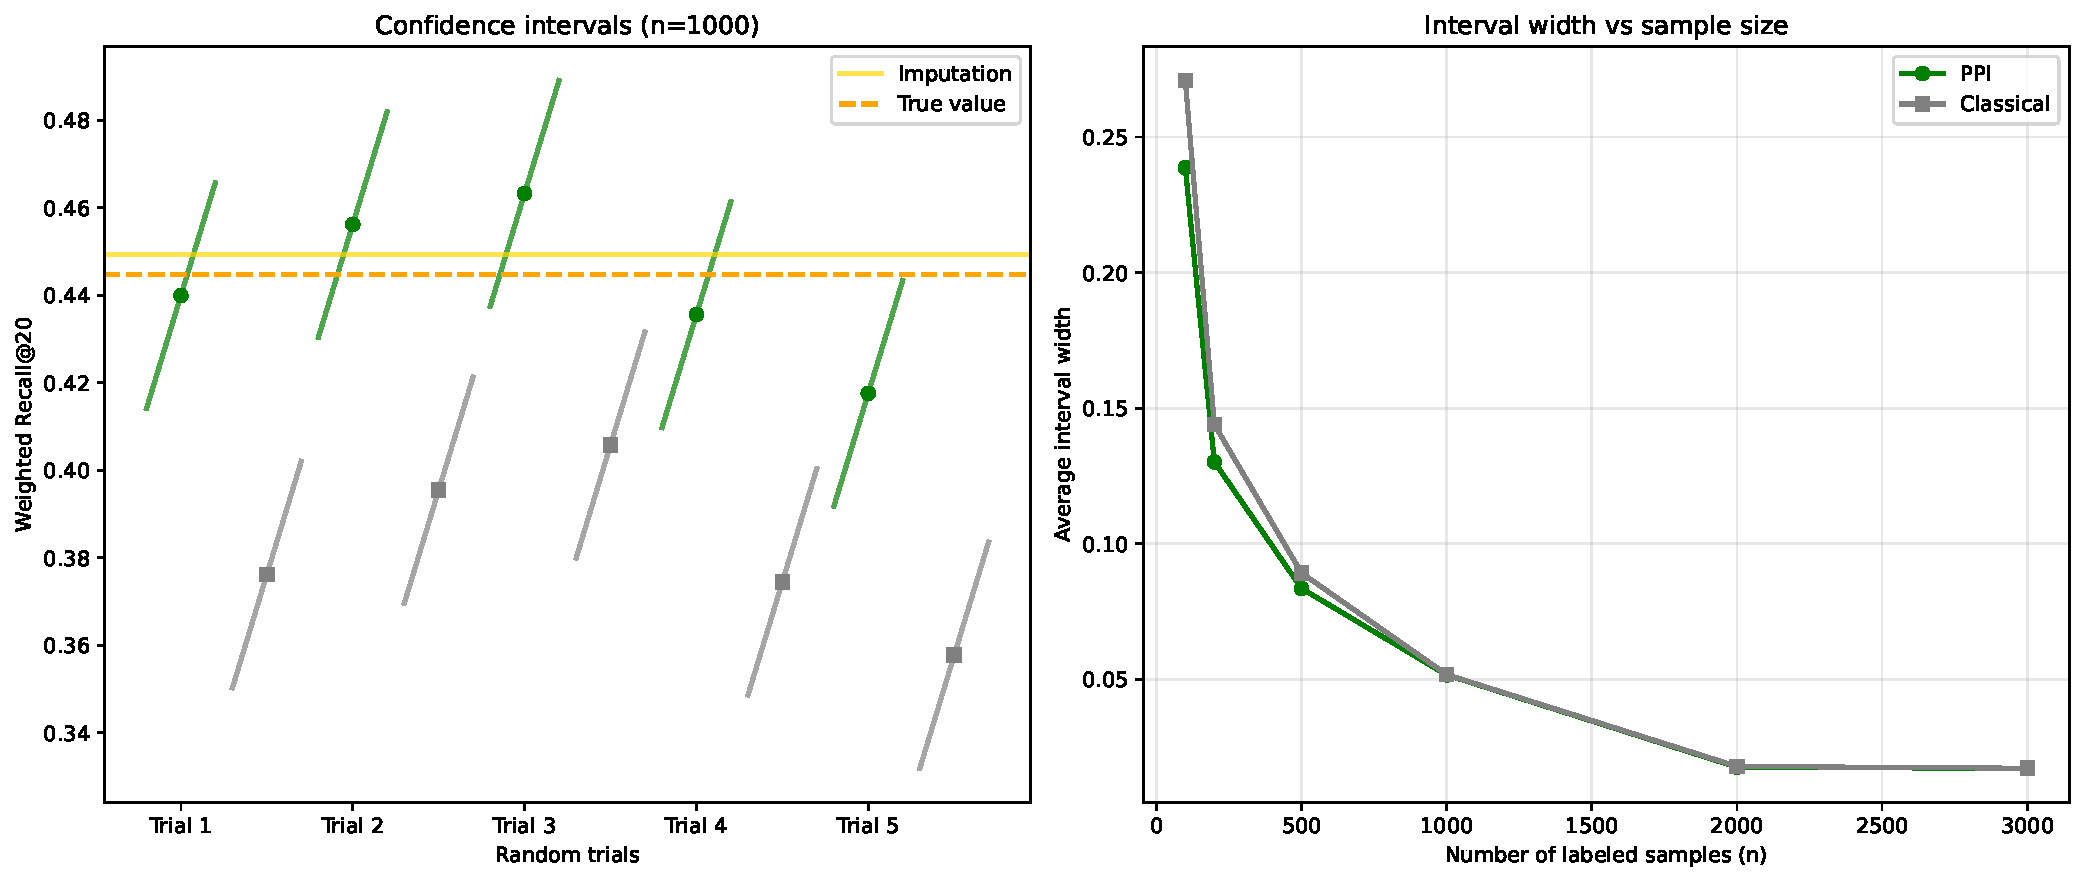
\includegraphics[width=0.9\textwidth]{images/comparison_plot.pdf}
\caption{PPI, 经典方法与填补法的估计结果对比}
\label{fig: comparison_plot}
\end{figure}

从图~\ref{fig: comparison_plot} 可以看出, PPI方法构造的置信区间具有良好的覆盖性质. 以$n=1000$为例, 经典方法与填补法均有未能覆盖真实值的情况, 但PPI方法能够覆盖全部真实值. 事实上, 通过计算发现, PPI置信区间在不同标注样本量下均能覆盖真实值, 而经典方法在$n=100, 200, 500, 1000$时均未能覆盖真实值, 直到$n=2000$后才开始覆盖. 填补法则完全依赖于预测模型的质量, 在本实验中其点估计虽然接近真实值, 但未能反映预测偏差带来的不确定性. 

从区间宽度来看, PPI方法同样优于经典方法. 观察图~\ref{fig: comparison_plot} 可知, 在不同的标注样本量下, PPI方法给出的置信区间宽度都比经典方法给出的区间宽度更窄. 出现这个优势的原因在于, PPI方法会利用大规模未标注的数据来降低估计量的方差, 同时还能通过校正量来保持无偏性. 当预测模型比较准确的时候, PPI估计量的方差将主要由$\frac{1}{n}\mathrm{Var} (e_i) $决定, 这个数值会远小于经典方法中的$\frac{1}{n}\mathrm{Var} (Y_i) $. 

由此, 本研究验证了PPI方法在推荐系统数据集中的有效性. 

\section{基于PPI方法的召回策略选择}

前文的实验已经验证了PPI方法可以用来估计加权召回率. 对于传统的方法来说, 模型大多只能计算得到点估计值, 很难判断出策略之间的差异到底是否来源于随机波动; PPI方法则有所不同, 它给出的置信区间能为这种比较提供统计上的依据. 这里就能引出一个自然延伸的问题, 能否把PPI方法当作合适的评估工具, 更全面地比较不同召回策略的优劣情况? 为了探讨这一问题, 本节会把PPI方法用到六种召回策略的性能评估上, 展现其在推荐系统离线评估环节中的实际价值. 

\subsection{六种常规召回策略}

本文采用了六种常规召回策略, 每种策略对应着不同的候选物品生成方式. 历史行为策略\upcite{Linden2003}仅基于会话历史序列中的物品进行加权打分, 权重由行为类型与位置衰减共同决定. 邻域传播策略\upcite{Wang2020}通过共现矩阵进行多层邻居传播, 将点击, 加购与购买的传播权重分别设为0.8, 0.6与0.4, 传播层数设为3层, 每层锚点数量限制为8个. 转移矩阵策略\upcite{Rendle2010}利用点击到加购, 加购到购买的转移矩阵扩展候选物品, 转移权重分别设为0.5与0.7. 类别相似策略\upcite{Pazzani2007}则基于物品类别推荐相似物品, 类别权重设为0.3. 此外还有长期兴趣策略\upcite{Yin2024}, 统计全局热门物品, 其中长期兴趣权重设为0.4. 融合策略将上述五种策略的得分加权求和后生成最终推荐列表. 所有策略的推荐列表长度统一设为$K=20$. 

\subsection{各召回策略的PPI估计结果}

实验评估了六种召回策略的PPI加权召回率, 由此对不同策略作出评价. 

以标注样本量$n=500$为例, 历史行为策略的加权召回率最高, 可达到0.4965, 置信区间为$[0.4414, \ 0.5517]$; 融合策略次之, 召回率为0.4449, 置信区间为$[0.3832, \ 0.5066]$; 其他几项策略的加权召回率都较低, 且与前两者的置信区间重叠度为0, 差异显著, 召回效果不佳. 具体对比如图~\ref{fig: strategy_comparison} 所示. 
\begin{figure}[htbp]
\centering
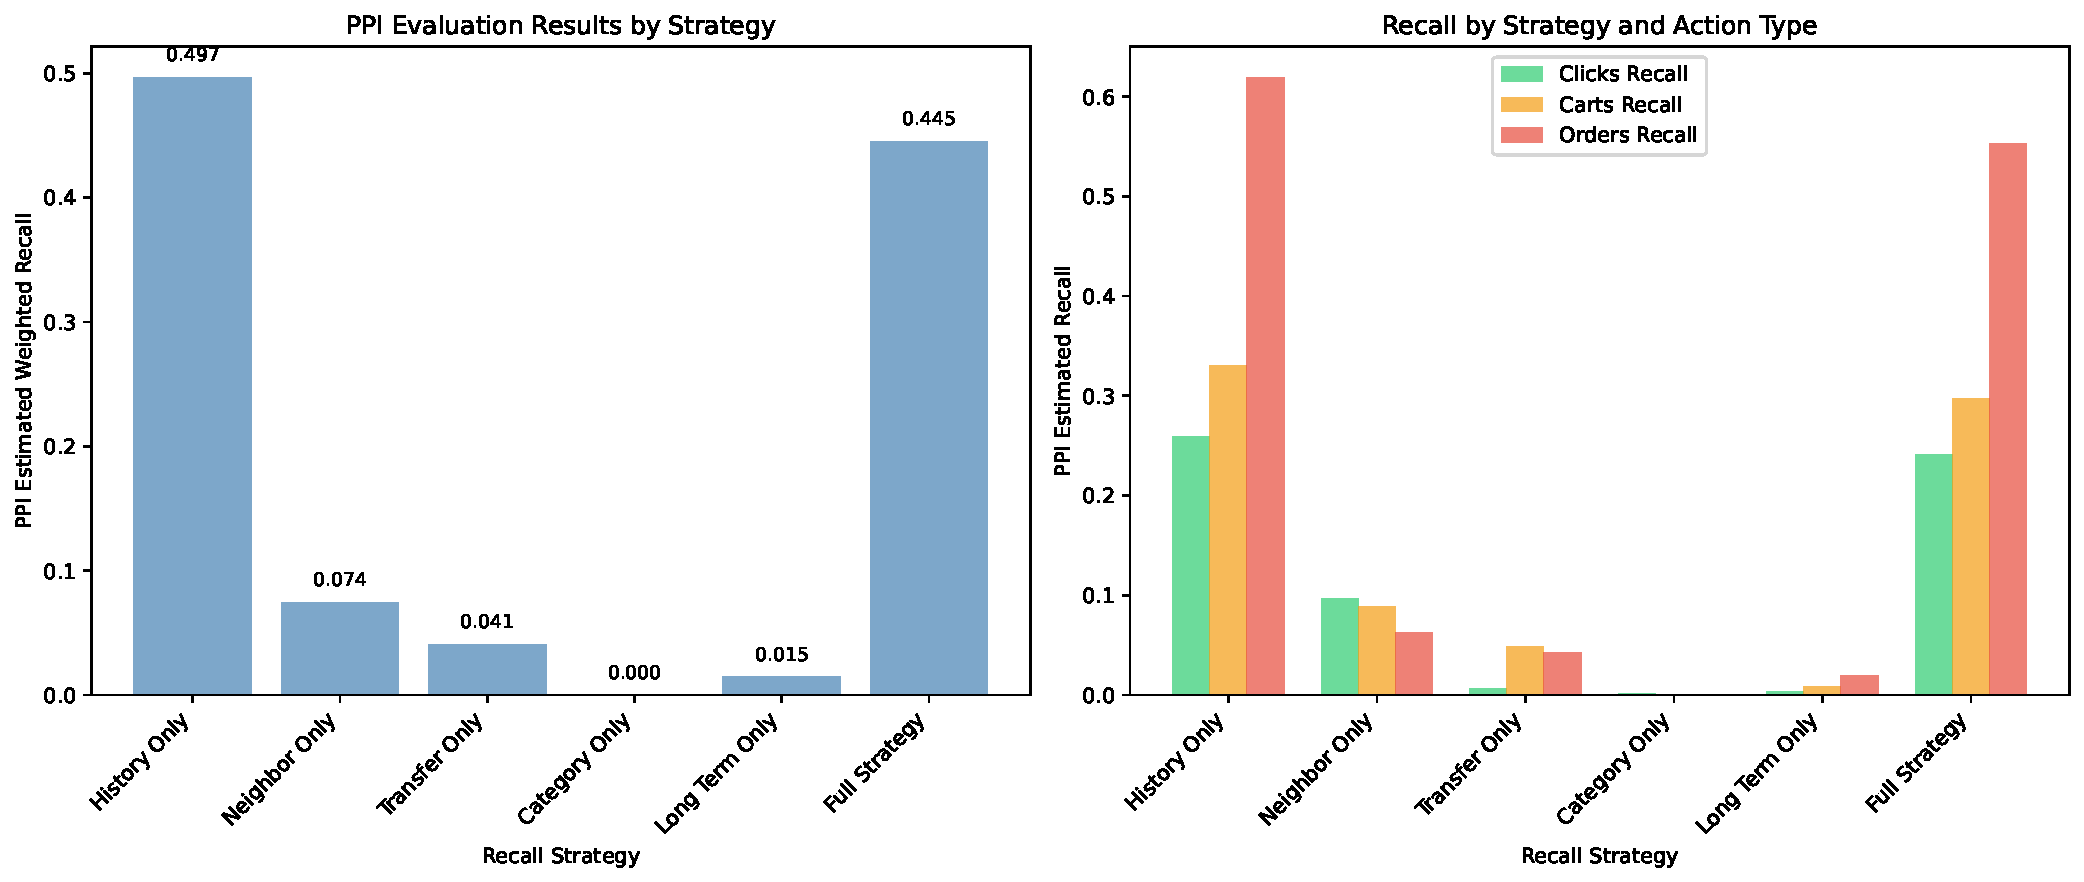
\includegraphics[width=0.8\textwidth]{images/strategy_comparison.pdf}
\caption{六种召回策略的PPI评估结果对比}
\label{fig: strategy_comparison}
\end{figure}

从图~\ref{fig: strategy_comparison} 可以看出, 在两种效果比较好的策略中, 购买行为的召回率普遍高于点击和加购行为, 这可能与购买行为的数据稀疏性和业务重要性有关. 其中, 历史行为策略在购买行为上的召回率更是高达0.6192, 远高于其在点击 (0.2594) 和加购 (0.3303) 上的表现. 融合策略虽然在加权召回率上略低于历史行为策略, 但与历史行为策略的置信区间大幅重叠, 两者在统计上没有显著差异. 


\subsection{最优策略选择与原因分析}

以加权召回率为核心指标, 本研究最终将把历史行为策略选定为最佳策略, 这一点可以从推荐系统的行为模式角度进行解释. 在OTTO数据集中, 用户的历史行为序列本身就已经包含了比较丰富的偏好信息, 因此基于历史物品的加权推荐能够更加有效捕捉用户的短期兴趣. 相比之下, 融合策略虽然综合了多种信息源, 但不同信号之间的权重分配可能存在优化空间, 简单的加权融合反而稀释了强信号的贡献. 这一发现对召回策略的设计具有重要启示: 在资源有限的情况下, 优先优化历史行为策略可能比追求复杂的多源融合更为高效. 

\section{数据特征对PPI方法的影响}

前文的实验验证了PPI方法在召回策略评估中的有效性. 不过, 评估结果的可靠性往往与数据特征有着紧密的联系. 在实际的推荐系统中, 用户行为数据的分布往往会呈现出比较复杂的变化模式, 有可能对PPI的估计结果产生干扰. 因此, 本节将从会话长度和时间窗口两个维度出发, 探究数据特征会如何影响PPI的评估效果, 从而为后续分布漂移问题的讨论奠定基础. 

\subsection{会话长度对PPI估计的影响}

实验2把验证集里的会话按照长度划分成三组, 一组是短会话 (事件数小于10, 一共有1468个), 一组是中等会话 (事件数在10到30之间, 一共有992个), 还有一组是长会话 (事件数大于30, 一共有1540个). 每一组会随机抽取出300个会话作为标注数据代入PPI估计, 以此探究会话长度对PPI估计值的影响. 图~\ref{fig: session_length} 揭示了不同会话长度下PPI方法计算得出的加权召回率. 

\begin{figure}[htbp]
\centering
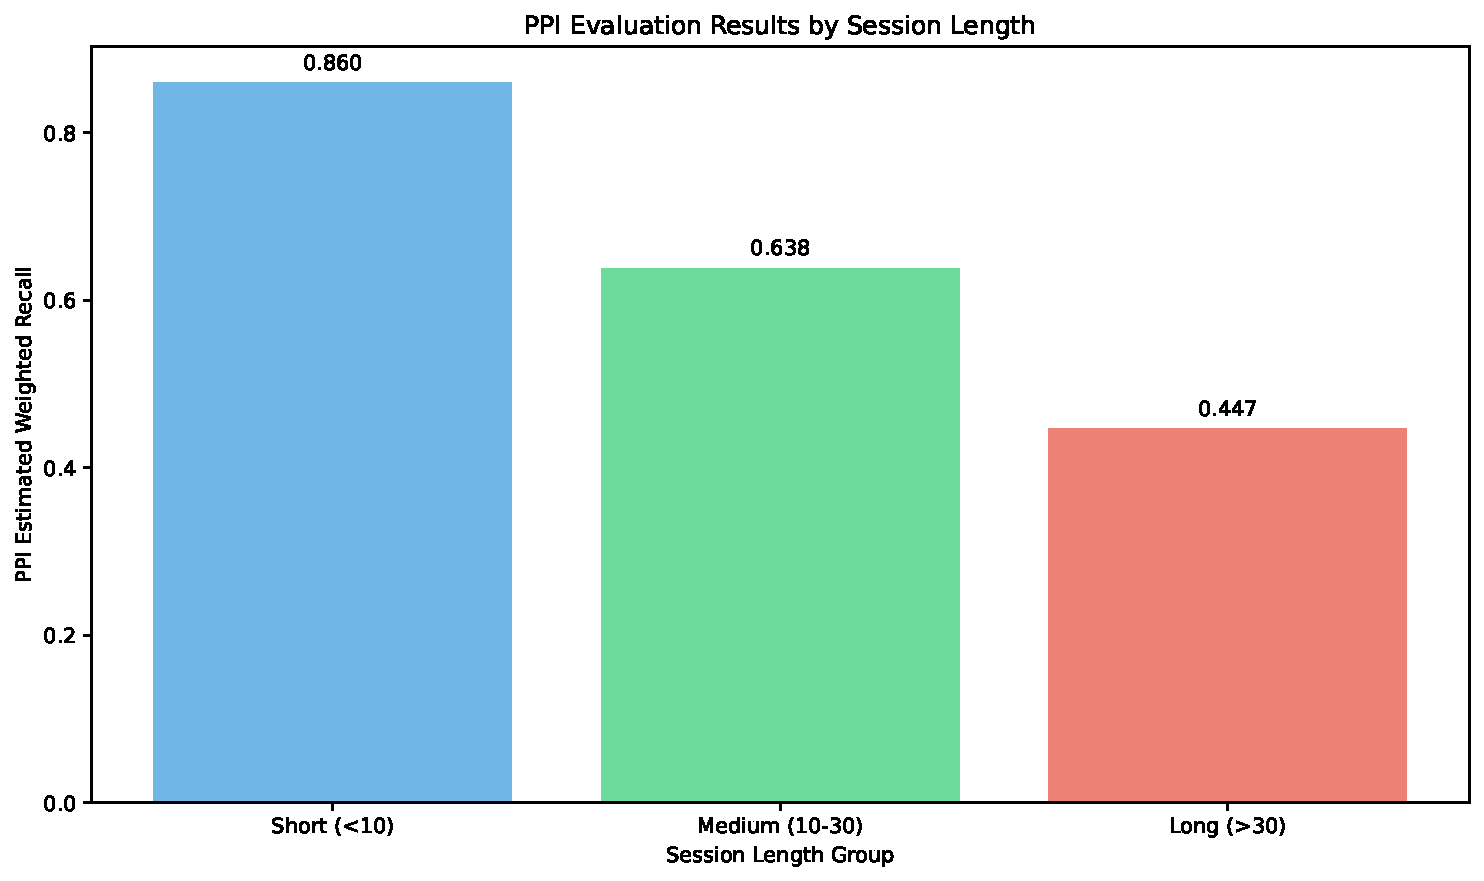
\includegraphics[width=0.6\textwidth]{images/session_length_comparison.pdf}
\caption{不同会话长度分组的PPI评估结果 (含95\%置信区间) }
\label{fig: session_length}
\end{figure}

如图~\ref{fig: session_length} 所示, 短会话的加权召回率最高, 中等会话次之, 长会话最低. 计算可得, 短会话的95\%置信区间为$[0.217, 0.903]$, 中等会话的置信区间为$[0.541, 0.736]$, 长会话的置信区间为$[0.389, 0.504]$. 其中, 中等会话与长会话的置信区间互不重叠, 两组之间的差异在统计上显著. 由此可以说明会话长度对召回效果的影响并非随机波动, 而是具有统计意义的系统差异. 这一现象可以从两个角度解释. 一方面, 短会话中的用户意图更为集中, 行为模式更为明确, 因此预测模型能够更准确地估计其召回率, 从而使得矫正量的方差较小. 另一方面, 长会话通常包含多种行为类型的混合, 用户兴趣可能发生多次转移, 增加了预测的难度. 

值得注意的是, 短会话的PPI置信区间宽度虽然最宽, 但购买召回率最高, 这表明对于行为序列极短的会话, 用户的购买意图非常明确, 推荐系统能够准确命中. 这一发现对推荐系统下的冷启动场景设计也具有启示意义: 对于新用户或行为稀疏的用户, 基于有限历史行为的简单策略可能比复杂模型更为有效. 

\subsection{时间窗口对PPI估计的影响}
实验将验证集按时间顺序划分为早, 中, 晚三个窗口, 每个窗口约占总会话数的三分之一, 分别包含1224, 1203和1220个有效会话. 每组随机抽取300个会话进行PPI估计, 由此探究时间变化对PPI估计量的影响. 

计算可得, 早期窗口的加权召回率可达0.521, 在三个窗口中最高; 晚期窗口次之, 中期窗口最低. 同时, 早期窗口下的95\%置信区间为$[0.444, 0.599]$, 中期窗口为$[0.356, 0.508]$, 晚期窗口为$[0.413, 0.567]$. 从置信区间的重叠情况来看, 早期窗口与中期窗口的重叠率为41.9\%, 表明两者之间存在一定程度的差异但不完全分离; 早期窗口与晚期窗口的重叠率高达79.9\%, 说明这两个窗口的估计结果在统计上较为接近; 中期窗口与晚期窗口的重叠率为62.0\%, 同样呈现部分重叠. 总体而言, 不同时间窗口上的PPI估计结果存在一定波动, 暗示数据分布可能随时间发生了缓慢变化. 具体对比如图~\ref{fig: time_window} 所示. 

\begin{figure}[htbp]
\centering
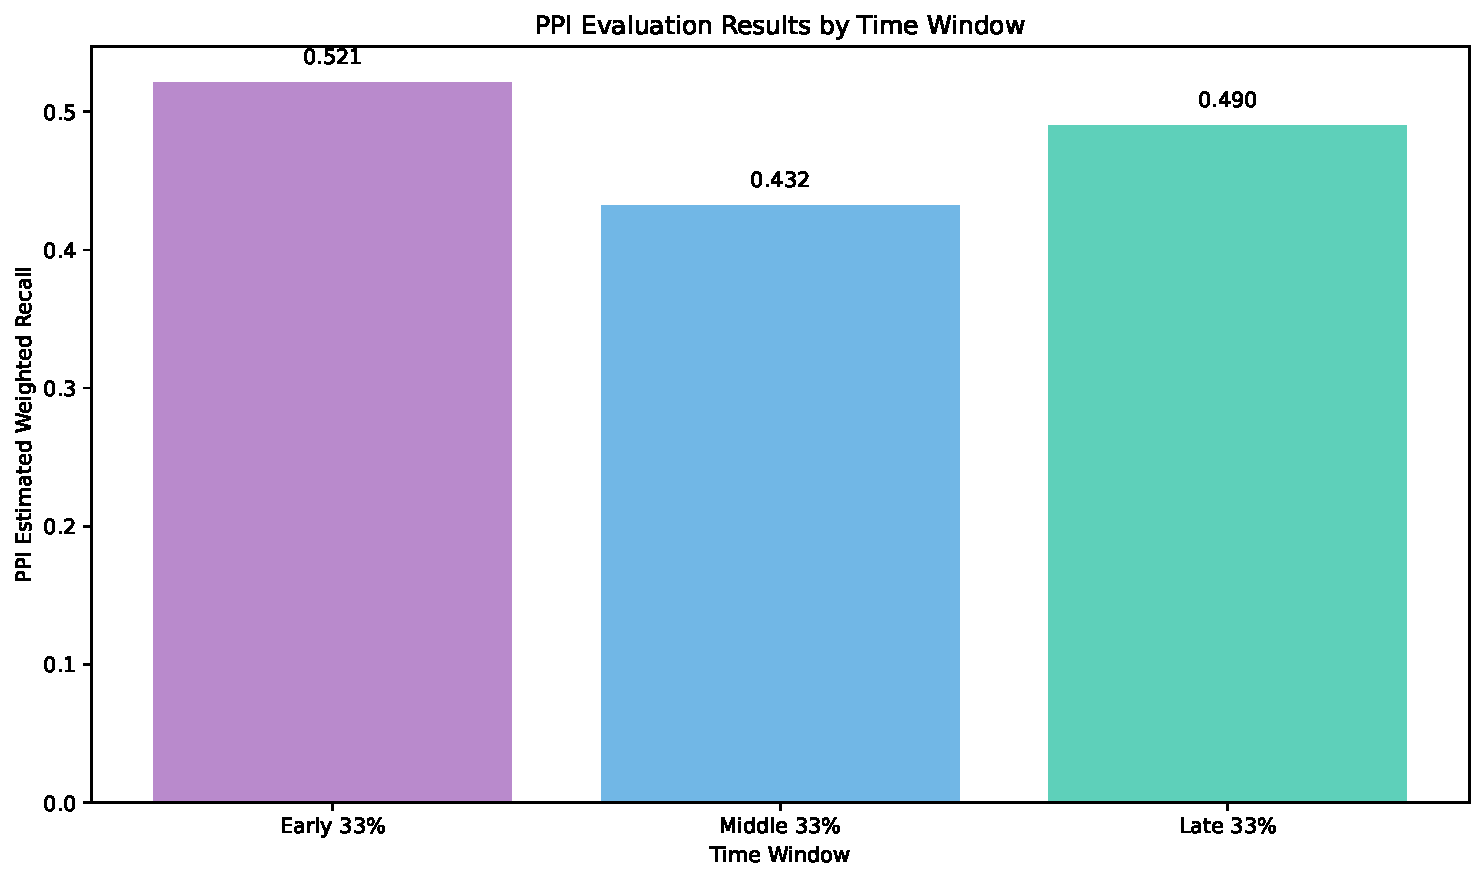
\includegraphics[width=0.7\textwidth]{images/time_window_comparison.pdf}
\caption{不同时间窗口分组的PPI评估结果 (含95\%置信区间) }
\label{fig: time_window}
\end{figure}

为什么数据特征会对PPI的估计结果产生影响? 它的本质原因能够归结于分布漂移. PPI方法的核心假设是标注数据与未标注数据都来自于同一个分布, 但当会话长度分布不均匀或者时间窗口发生了某些变化时, 这个假设就很有可能不成立. 训练集和验证集之间的分布差异会导致标准PPI估计产生偏差, 因此检测并且校正分布漂移是确保PPI方法能够在复杂数据环境下有效应用的关键. 

\section{分布漂移下的预测驱动推断}

上一节的内容表明, 会话长度和时间窗口这类数据特征会影响PPI的估计结果, 而其本质原因是标注数据与目标数据之间存在分布漂移. 本节引入了三种比较典型的分布漂移: 协变量漂移, 标签漂移与时间漂移, 并且给出了相应的校正方法. 通过区分不同的漂移类型, 本研究可以更加精准地定位PPI估计偏差的来源, 从而提升校正方法的针对性与有效性. 在具体分析之前, 本研究会先对三种分布漂移作出检测, 这样就能为后续的校正策略提供明确的诊断依据. 

\subsection{协变量漂移与加权PPI校正}

在协变量漂移的检测中, 可通过会话长度分布计算出重要性权重$w (x) =Q_X (x) /P_X (x) $. 检测结果如图~\ref{fig: covariate_shift_analysis} 所示, 权重范围在0.51到1.13之间, 最大值与最小值的比值约为2.22, 这就表明存在着明显的协变量漂移, 需要引入重要性加权PPI进行校正. 与标准PPI相比, 重要性加权PPI有效缩减了约27\%的估计偏差, 它的置信区间也能够成功覆盖真实值, 保证了校正策略的可靠性. 

\begin{figure}[htbp]
\centering
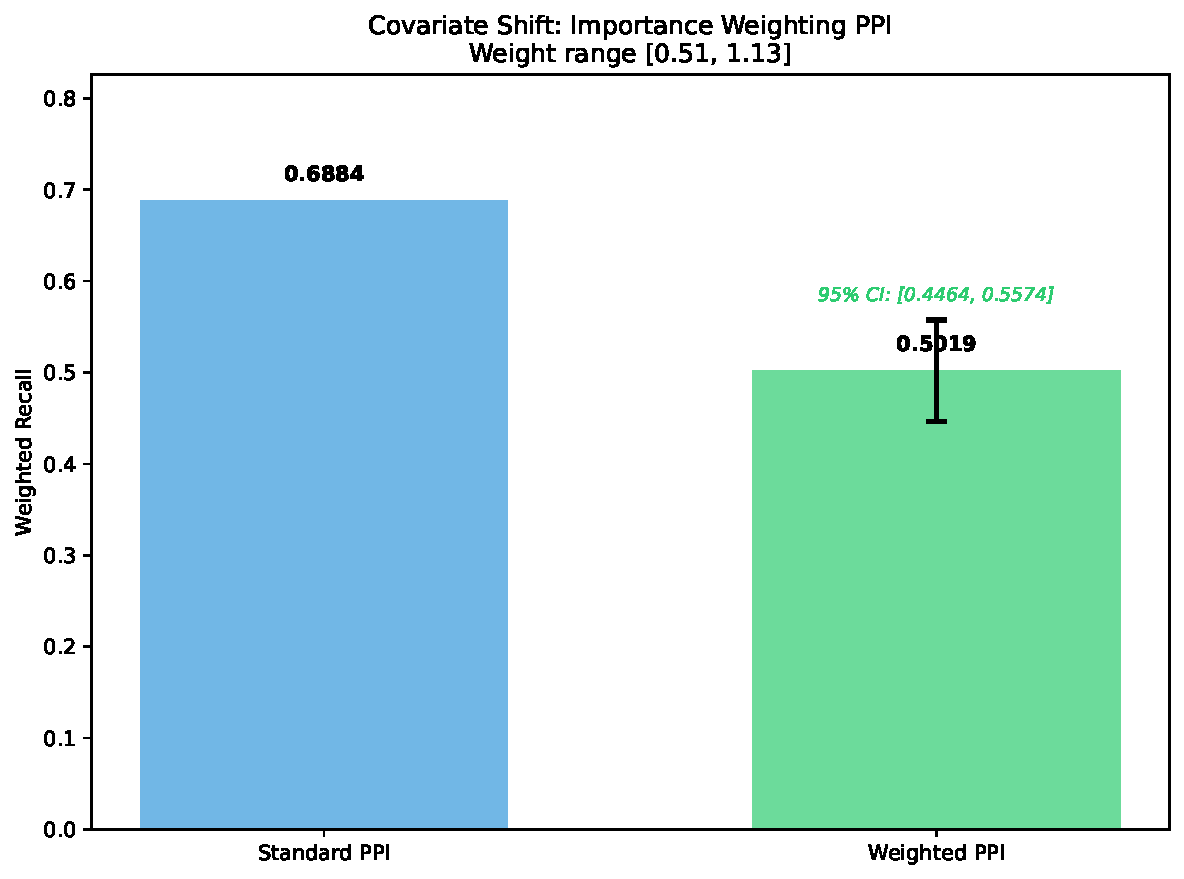
\includegraphics[width=0.7\textwidth]{images/covariate_shift_analysis.pdf}
\caption{协变量漂移检测结果}
\label{fig: covariate_shift_analysis}
\end{figure}

这一发现表明, 当标注数据与未标注数据的特征分布有明显不同时, 如果不进行校正, 标准PPI的估计会严重偏离真实值. 通过引入重要性权重校正协变量漂移, 加权PPI能够有效减少这种偏差, 提高预测的准确率. 

\subsection{标签漂移与混淆矩阵校正}

在标签漂移检测中, 可以比较训练集和验证集中三类行为的分布差异. 训练集分布为点击0.916, 加购0.068, 购买0.016, 验证集分布为点击0.915, 加购0.067, 购买0.018, 漂移幅度约为0.001, 变化较小. 混淆矩阵$\hat{\mathcal{K}}$的对角线元素均在0.89以上, 表明预测模型具有较高的分类准确率. 图~\ref{fig: label_shift_analysis} 给出了标签漂移的检测结果. 

\begin{figure}[htbp]
\centering
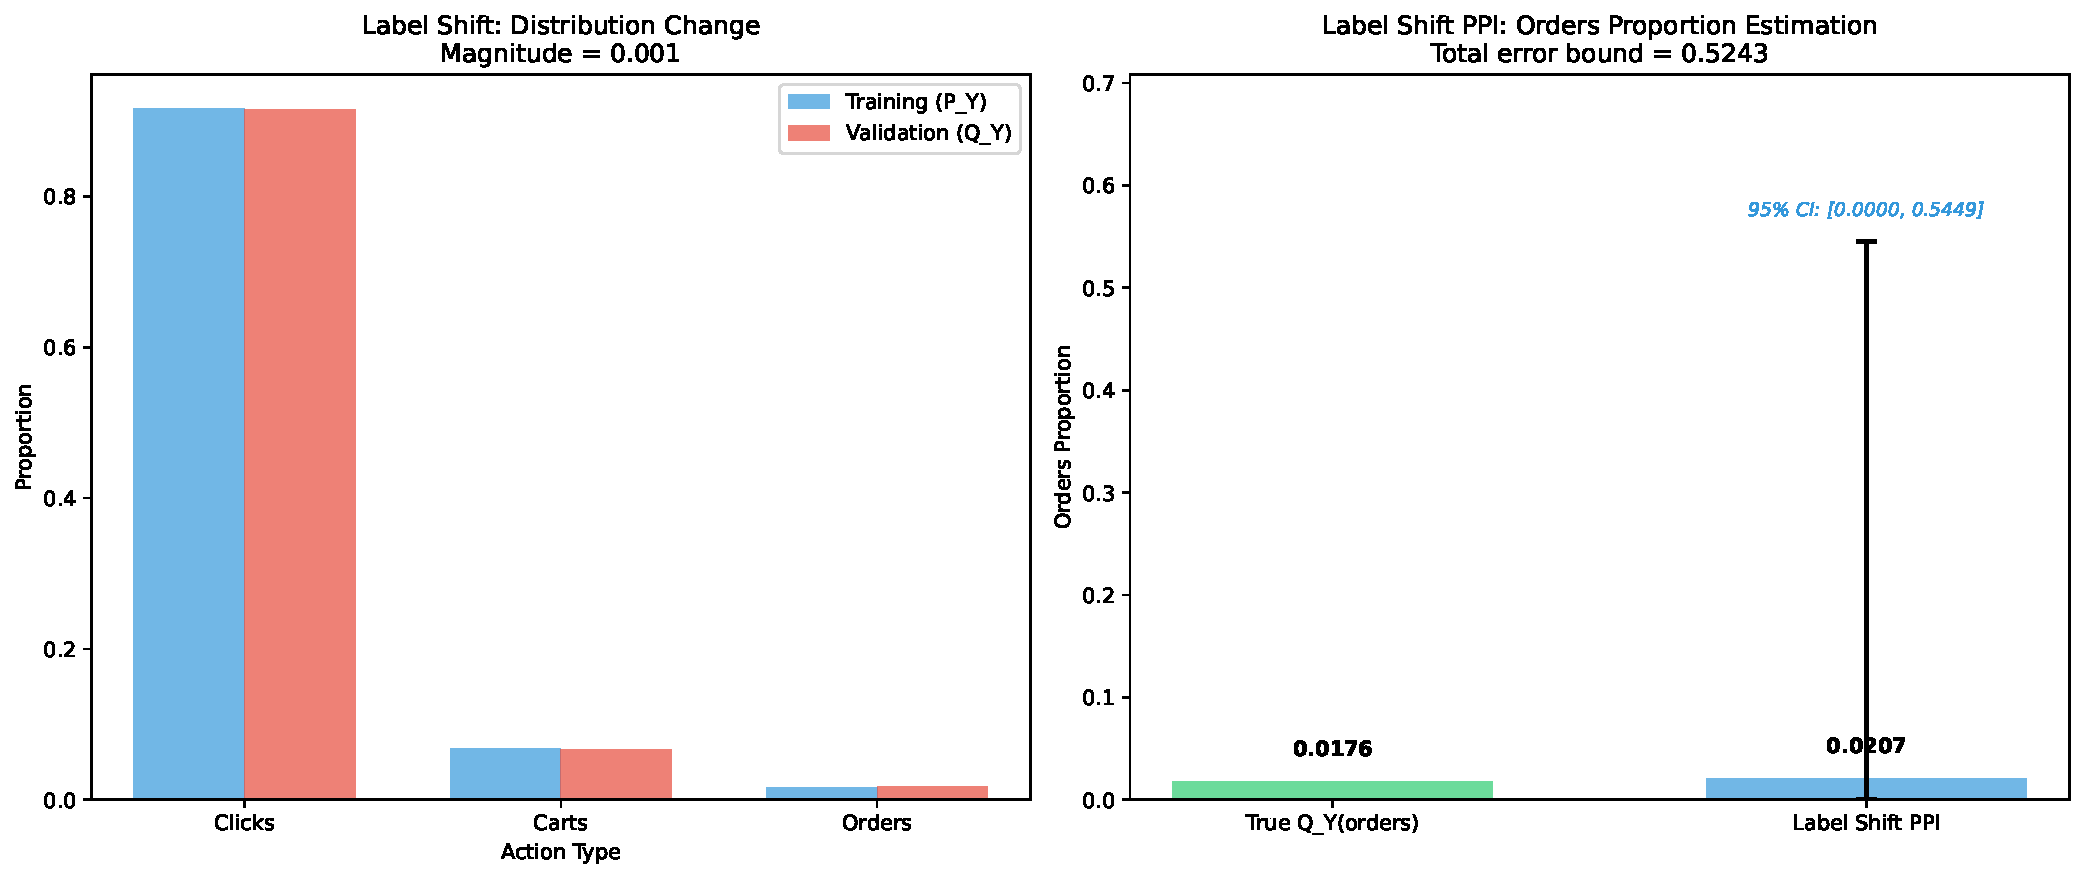
\includegraphics[width=0.8\textwidth]{images/label_shift_analysis.pdf}
\caption{标签漂移检测结果}
\label{fig: label_shift_analysis}
\end{figure}

如图~\ref{fig: label_shift_analysis} 所示, 本实验中几乎不存在标签漂移. 尽管如此, 在实际应用中, 混淆矩阵校正方法仍能有效估计真实标签分布. 当标签漂移较为显著时, 该方法的重要性将更加突出. 

\subsection{时间漂移与滑动窗口PPI校正}

研究将会话按时序划分为6个窗口, 每个窗口约500个会话. 图~\ref{fig: time_shift_analysis} 给出了时间漂移的检测结果. 
\begin{figure}[htbp]
\centering
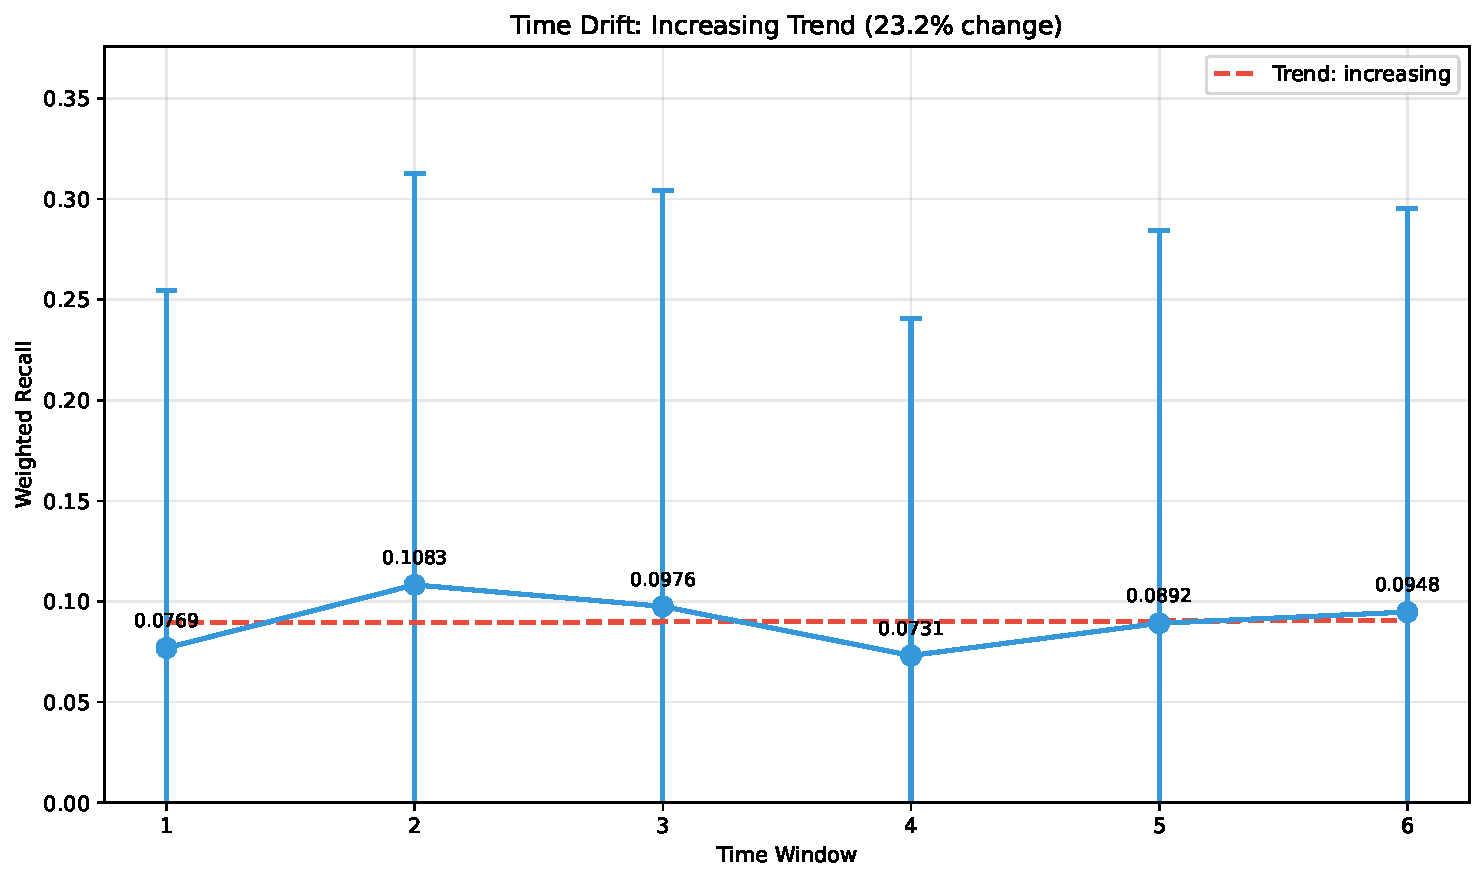
\includegraphics[width=0.7\textwidth]{images/time_drift_analysis.pdf}
\caption{时间漂移检测结果}
\label{fig: time_shift_analysis}
\end{figure}

如图~\ref{fig: time_shift_analysis} 所示, 窗口加权召回率呈现波动趋势, 最终变化幅度达23.2\%, 表明存在一定程度的时间漂移. 针对该问题, 本文将引入滑动窗口PPI进行校正. 计算得出, 滑动窗口PPI和加权滑动窗口PPI的估计值都与标准PPI相近, 但置信区间的宽度有所增大. 这一现象并非说明时间漂移校正方法本身无效, 而是与本数据集中时间漂移的具体方向有关. 滑动窗口方法赋予近期数据更高的权重, 而实验数据显示近期会话的加权召回率整体偏低, 因此校正后的估计值出现向下偏移. 此外, 时间窗口的划分会导致有效样本量减少, 这也是置信区间宽度增大的重要原因. 


\subsection{最优校正方法}
综合而言, 重要性加权PPI取得了更好的校正效果. 由于标签漂移在本数据集上并不显著, 混淆矩阵方法的改善作用不大. 而滑动窗口方法的有效性取决于时间漂移的方向与幅度, 在更长时序跨度或漂移方向稳定的数据中可能发挥更大作用. 

\section{集成预测驱动推断的性能分析}

除了数据因素之外, 预测模型本身的性能同样对PPI方法的应用效果起着决定性作用. 单一模型的预测能力往往有限, 因此, 本节将探讨集成学习框架下三种PPI变体的性能, 并以单一PPI模型作为基线进行对比. 

\subsection{集成方法的点估计与置信区间}

本节在六种标注样本量 ($n=100, 200, 500, 1000, 2000, 3000$) 下分别运行8次重复实验, 对比四种方法的估计性能. 对8次实验结果取平均. 表~\ref{tab: ensemble_summary} 汇总了四种PPI方法在所有样本量和所有重复实验下的加权召回率均值, 标准差及95\%置信区间. 

\begin{table}[H]
\centering
\caption{四种PPI方法的加权召回率统计汇总}
\label{tab: ensemble_summary}
\begin{tabular}{lcccc}
\hline
方法 & 加权召回率均值 & 标准差 & 95\%置信区间下限 & 95\%置信区间上限 \\
\hline
单一 PPI & 0.4282 & 0.0639 & 0.2832 & 0.5568 \\
Bagging PPI & 0.4388 & 0.0354 & 0.3482 & 0.5028 \\
Stacking PPI & 0.4440 & 0.0464 & 0.3600 & 0.5166 \\
Cross-PPI & 0.4462 & 0.0526 & 0.3156 & 0.5520 \\
\hline
\end{tabular}
\end{table}

从表~\ref{tab: ensemble_summary} 可以看出, 三种集成方法在加权召回率估计的准确性和稳定性方面均优于单一PPI方法, 验证了集成策略在召回评估中的有效性. 

在准确性方面, 所有集成方法的加权召回率都比单一PPI方法更接近真实值 (0.4447). 其中, Cross-PPI和Stacking PPI的结果最接近真实值, 较单一PPI提升了最多. 这说明, 采用交叉验证方式和自适应权重来训练基模型能够有效地降低估计的偏差. 此外, Bagging PPI方法也取得了一定提升. 

在估计稳定性方面, 集成方法的优势同样十分突出. 单一PPI的标准差为0.0639, 置信区间宽度达到0.2736, 反映出该方法受单一预测器质量波动的影响较大. 相比之下, Bagging PPI的标准差降至0.0354, 置信区间收窄至0.1546, 收窄幅度超过43\%, 表明通过Bootstrap采样和模型平均能够显著降低估计方差. Stacking PPI同样表现出良好的稳定性, 其置信区间宽度为0.1566, 与Bagging PPI相当. Cross-PPI的置信区间宽度为0.2364, 虽然较前两者略宽, 但相比单一PPI仍有约14\%的收窄. 

\begin{figure}[htbp]
\centering
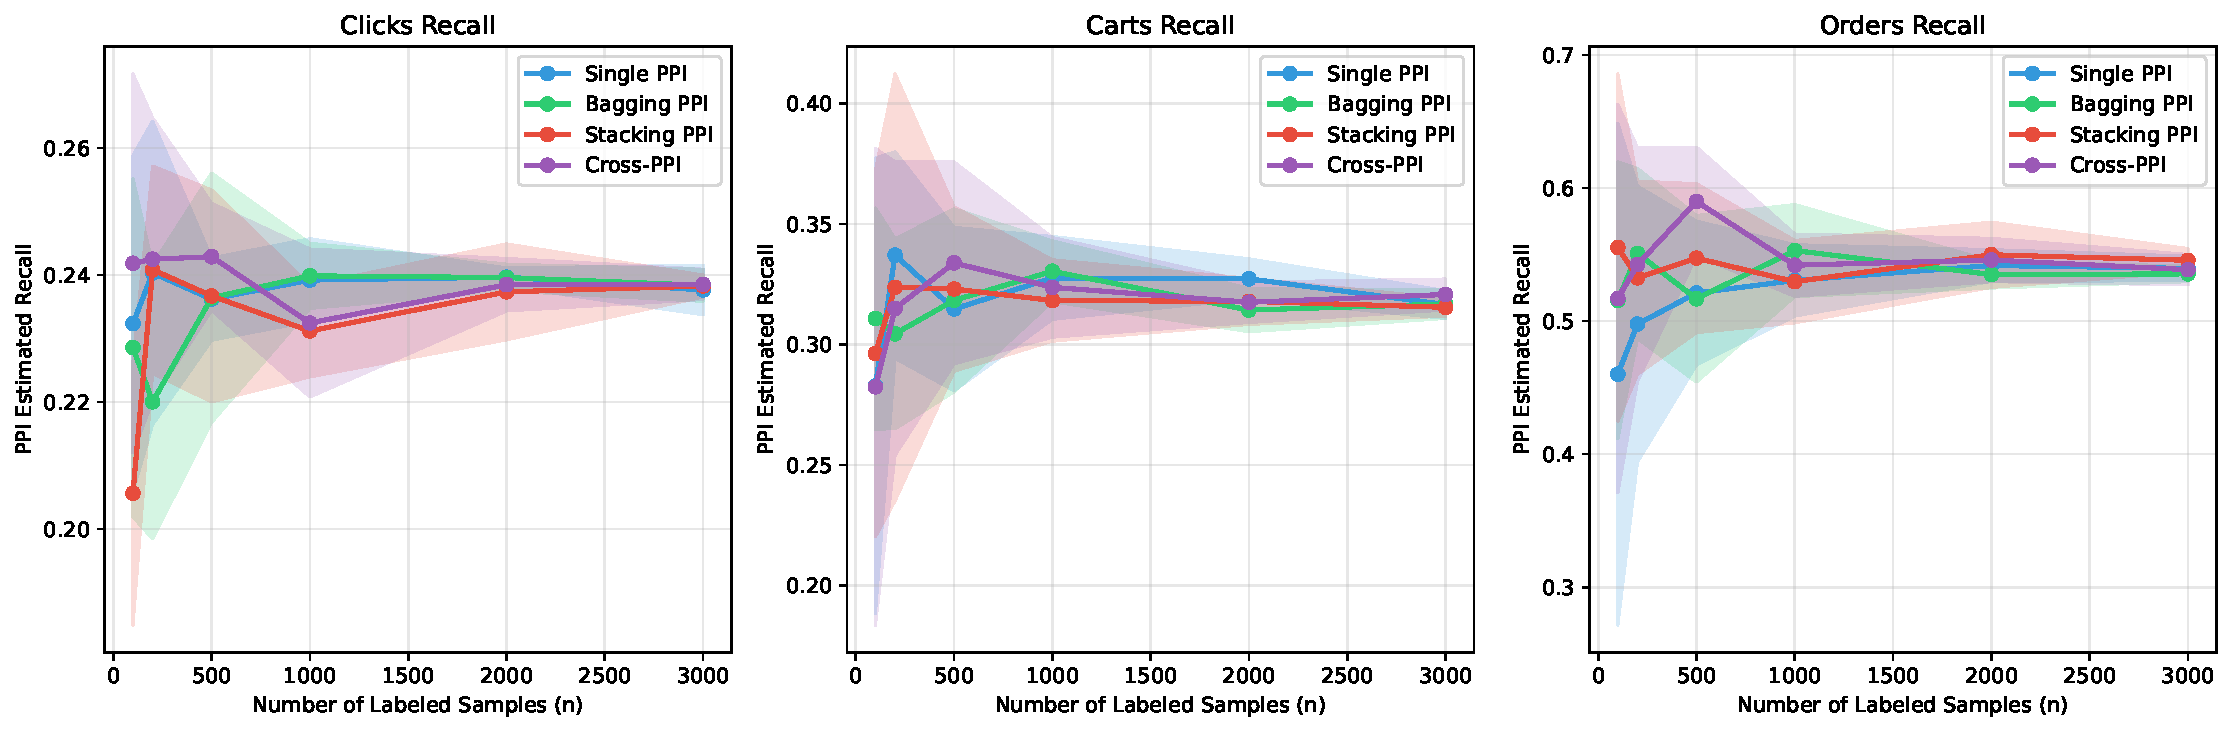
\includegraphics[width=0.8\textwidth]{images/ensemble_method_comparison.pdf}
\caption{不同PPI方法的召回率随标注样本量的变化趋势}
\label{fig: ensemble_trend}
\end{figure}


图~\ref{fig: ensemble_trend} 展示了四种方法的不同召回率随标注样本量$n$增加的变化趋势, 分别按点击召回率, 加购召回率和购买召回率三个指标呈现. 可以看出, 在购买指标中, 三种集成方法的优势最为明显; 在小样本量下, Cross-PPI往往表现最优, 这种优势随着样本量的增大而削弱. 


\begin{figure}[htbp]
\centering
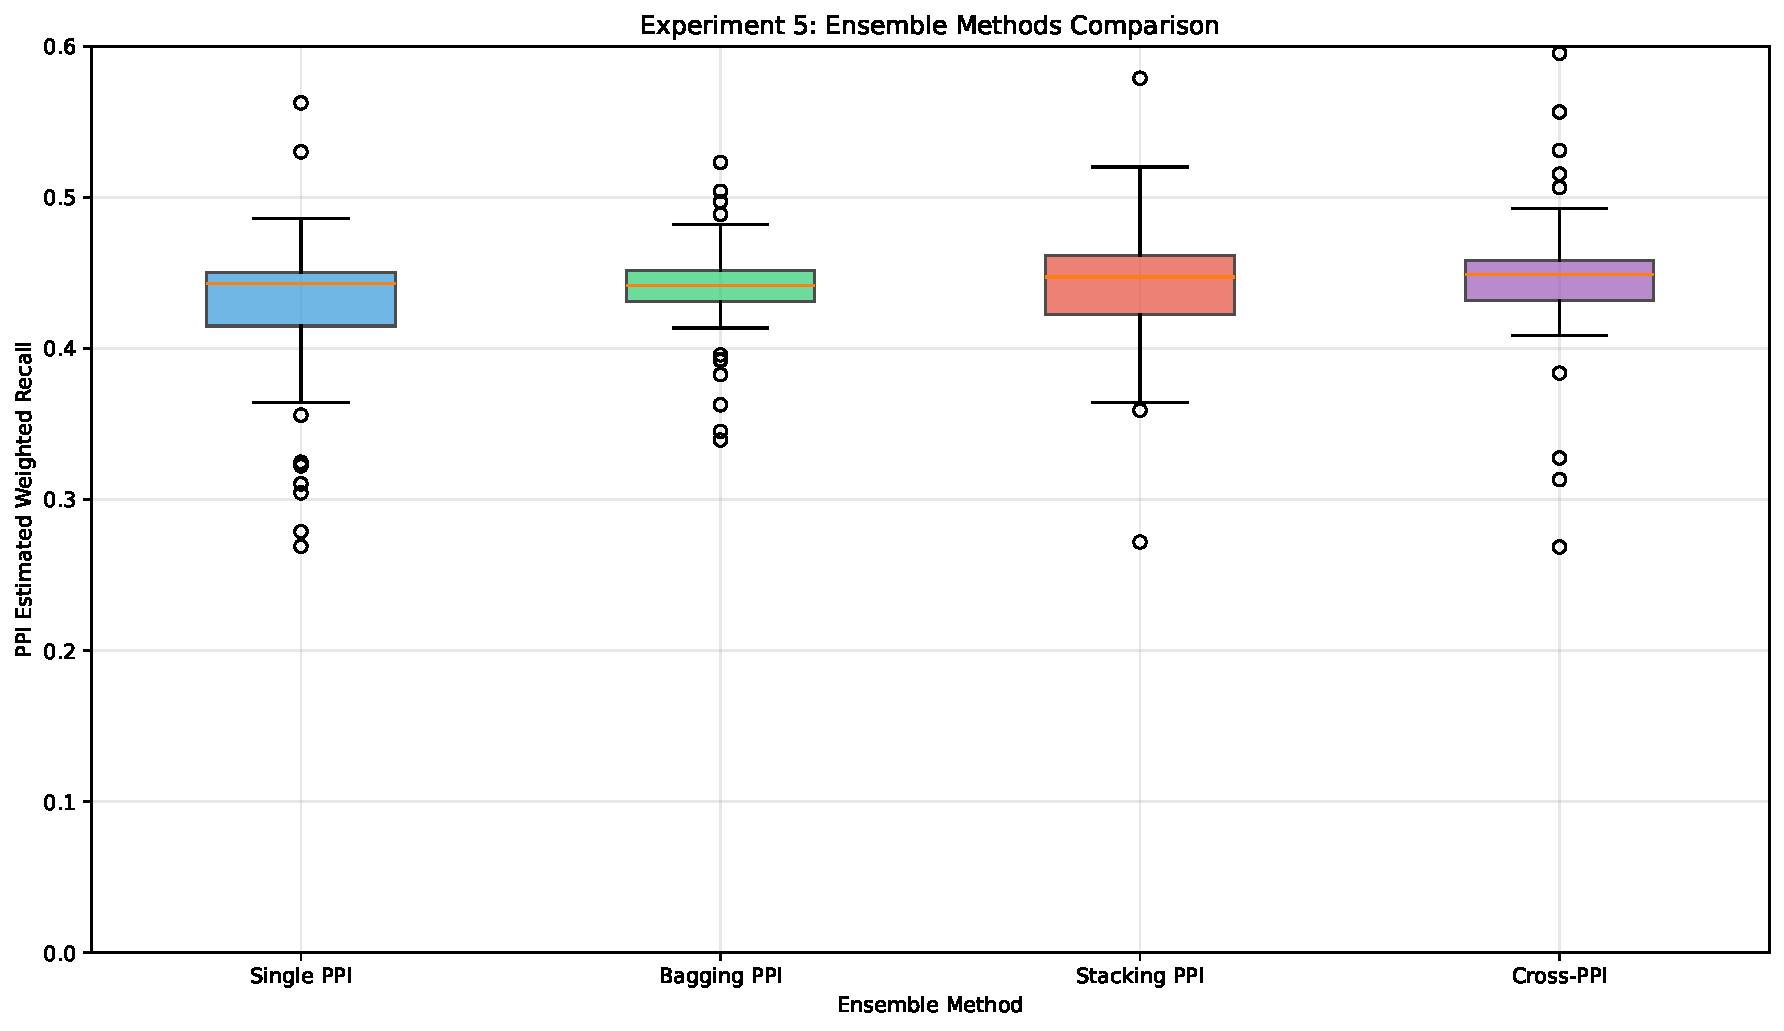
\includegraphics[width=0.8\textwidth]{images/ensemble_comparison_boxplot.pdf}
\caption{四种集成PPI方法的加权召回率箱线图对比}
\label{fig: ensemble_boxplot}
\end{figure}

图~\ref{fig: ensemble_boxplot} 则以箱线图的形式展示了四种方法在所有重复实验中的加权召回率分布情况, 箱体的高度反映了各方法估计值的离散程度. 可以看出, Bagging PPI的箱体最窄, 其估计结果最为稳定; Cross-PPI的箱体宽度适中, 稳定性次之; 单一PPI和Stacking PPI的箱体较宽, 波动较大. 

综合来看, 不同集成方法各有侧重: Cross-PPI在点估计精度上表现较好, 适合对估计准确性要求较高的场景; Bagging PPI则在区间估计的稳定性上更具优势, 适合需要更可靠的置信区间的应用场景. 单从准确性和计算开销的角度来看, 三种方法中Cross-PPI的表现最好; 引入均方误差来看, Bagging PPI在方差与偏差之间取得了更好的平衡. 实际应用中可根据具体需求选择合适的方法. 

综合上述结果可知, 集成策略能够在一定程度上有效提升预测驱动推断的估计性能. 


\subsection{效果分析}
Cross-PPI方法在估计精度上的优势可以从样本利用效率的角度进行解释. 与 Bagging-PPI 需要额外留出一个固定的校正子集不同, Cross-PPI 通过 $K$ 折交叉拟合的方式, 让全部 $n$ 个标注样本都能同时参与到模型训练和偏差校正的环节里, 不需要牺牲一部分样本来作为独立的校正集. 在标注样本量 $n$ 有限的情况下, 这种设计能够更充分地利用有限的数据信息, 进而提升矫正项的稳定性, 获得更准确的点估计. 实验结果显示, Cross-PPI的加权召回率均值在四种方法中最接近真实值, 可以验证这一优势. 

值得注意的是, Bagging-PPI 的标准差比 Cross-PPI 小, 出现这个情况的原因可能在于基模型训练数据量上的不同. Cross-PPI 会把原始数据划分为 $K$ 个互不重叠的子集, 每个基模型只能在大约 $1/K$ 的数据上作训练. 当 $K$ 较大时, 各基模型的训练数据量比较有限, 这就会导致基模型本身的预测方差 $\sigma_{\text{pred}}^2$ 增大. Bagging-PPI 的情况则有所不同, 每个基模型都在 Bootstrap 样本上训练, 数据量更加接近原始的数据量, 因此基模型会变得更稳定. 这样来看, Cross-PPI 虽然能够提高样本的利用效率, 但基模型自身方差的增大极有可能抵消这一优势. 

Stacking-PPI可以通过元学习器自适应地学习融合权重, 从理论上来看它能够获得比简单平均更好的融合效果. 不过, 在本次实验中, Stacking-PPI的改进幅度并不算很大, 这一结果可能与元学习器的训练数据量有限有关. 

从计算成本来看, Bagging-PPI和Cross-PPI的计算开销主要来自于基学习器的训练过程, 当$B=10$时集成模型的训练时间大约能到单一模型的10倍. Stacking-PPI还需要额外做一次交叉验证来训练元学习器, 所以它的计算成本会比前两者更高一些. 在实际的应用中, 需要根据计算资源和精度方面的要求去选择合适的集成方法. 

\section{冷启动场景的实验结果}

\subsection{冷启动场景下的特殊召回策略}

推荐系统在实际部署中常常会碰到冷启动问题\upcite{Schein2002}, 新用户或新物品没有足够多的历史交互数据, 常规的召回策略难以奏效. 为了缓解这个困境, 本文额外设计出了三类适用于冷启动场景的召回策略. 

聚类召回\upcite{Wang2020}会基于物品的共现模式构建出特征矩阵, 然后对物品进行聚类操作, 新物品会被分配到最相似的簇里, 再把这个簇里的热门物品取出来作为召回的结果. 

Look-alike召回\upcite{Liu2019}会构建出用户-物品的交互矩阵, 借助Jaccard相似度来计算用户之间的相似性, 找到与新用户行为模式比较相似的那些老用户, 再将老用户的偏好迁移过来作为新用户偏好的估计. 

双塔召回\upcite{Yi2019}采用典型的双塔模型结构, 用户塔以用户属性与历史行为为输入, 物品塔以物品内容特征为输入, 两者分别输出嵌入向量后通过内积计算匹配得分. 本文对标准双塔模型做了三方面改进: 引入偏差纠正层, 采用混合采样策略 (正样本权重设为2.0, 负采样比例设为0.3), 引入自监督学习辅助任务 (损失权重设为0.1). 模型训练采用Adam优化器, 初始学习率设为0.001, 权重衰减系数设为$10^{-5}$, 批处理大小为256, 训练轮数为8轮. 

\subsection{PPI在冷启动场景中的表现}

冷启动是推荐系统中的特殊场景, 极少量的交互行为会大幅降低推荐的准确性. 研究为此添加设置了上述三种召回策略及其混合召回. 图~\ref{coldstart} 显示了冷启动场景下的模型效果. 结果显示, 冷启动场景下PPI的应用效果仍然不佳, 预测质量普遍较低. 研究过程中, 基于内容特征的预测本身就存在较大偏差, 而PPI的效果高度依赖于预测模型的质量. 当预测模型不够准确时, 矫正量的估计方差较大, 反而可能引入额外的误差. 
\begin{figure}[htbp]
\centering
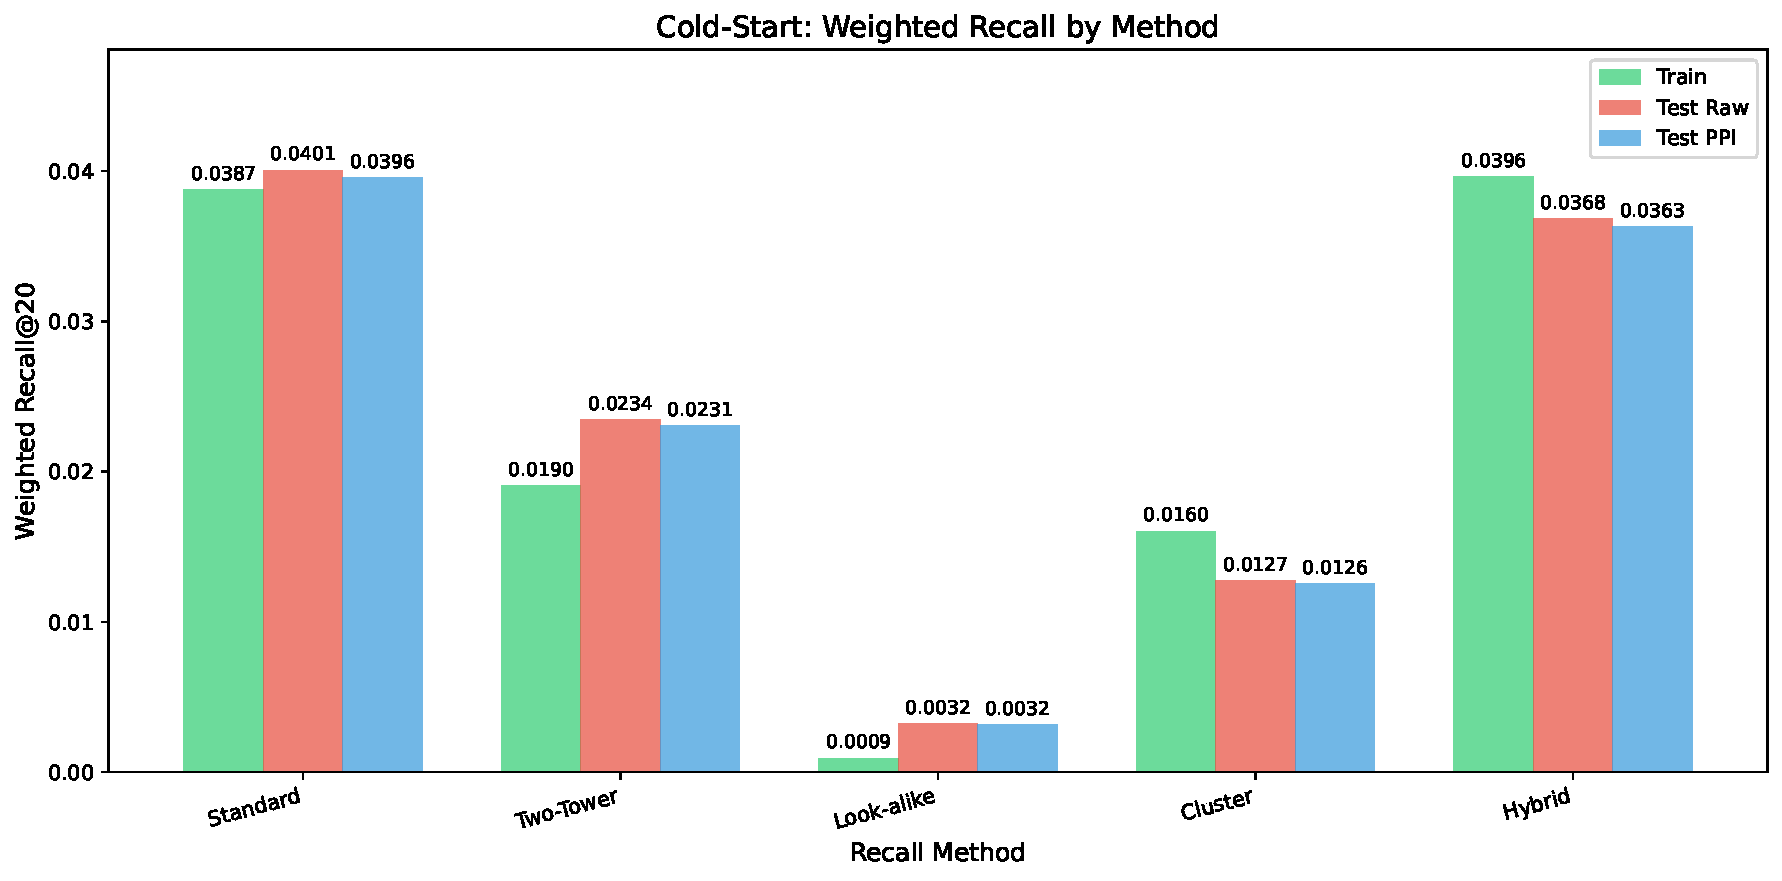
\includegraphics[width=0.9\textwidth]{images/cold_start_enhanced_comparison.pdf}
\caption{冷启动场景下的模型效果}
\label{coldstart}
\end{figure}

从图~\ref{coldstart} 可以看出, 常规召回方法及混合召回方法与PPI的结合效果稍好, 但总体召回率仍较低. 这一结果对冷启动场景下的PPI应用提出了警示: 在预测模型质量不足的情况下, 直接应用PPI可能无法获得预期的改善效果. 这也与前文发现形成呼应, 当单一模型预测能力有限时, 集成学习可以提升PPI性能; 但当预测质量低到一定程度时, 即使集成方法也可能难以奏效. 

在未来的研究中, 可以探索如何结合主动学习策略, 在冷启动场景下更加高效地获取标注数据, 提升预测模型的质量. 




\section{小结}

本章通过一系列实验系统地验证了预测驱动推断方法在推荐系统召回评估中的有效性, 同时从数据特征, 模型结构与应用场景这三个维度剖析了有可能影响PPI估计效果的关键因素. 


PPI与经典方法及填补法的对比实验表明, 该方法能够在保证置信区间覆盖概率的前提下, 有效地提升点估计精度与样本利用效率. 在此基础上, 召回策略评估进一步展示出了PPI在实际策略比较里所具有的应用能力, 它所构造出来的置信区间能够为不同策略之间的性能差异提供一个可量化的比较依据. 

在数据特征层面, 会话长度与时间窗口的相关分析揭示出数据分布差异会给估计结果带来明显的影响, 这种影响的本质能够归结为分布漂移问题. 针对这个问题, 本文介绍了协变量漂移, 标签漂移与时间漂移这三类典型情形, 并且给出了相应的校正方法. 

在模型结构层面, 集成PPI实验表明, 多模型融合策略能够进一步提升PPI的估计性能, 可以根据实际情况来选择不同的集成方法. 

在应用场景层面, 冷启动实验的结果揭示出PPI的估计效果会高度依赖于预测模型的质量, 当预测性能比较差的时候, 这种方法就很难获得预期的收益. 

这些方法可以为PPI框架在推荐系统里的离线评估应用提供参考. 

\chapter{总结与展望}

\section{研究总结}

本文围绕预测驱动推断方法在推荐系统召回评估中的应用展开研究, 同时把这个方法与集成学习结合到一起, 从数据特征, 模型结构与应用场景三个维度分析了有可能会影响推断效果的关键因素. 通过在OTTO推荐系统数据集上的实验, 本文验证了预测驱动推断方法在推荐系统离线评估中的有效性与实用价值. 

在方法层面上, 本文把召回评估问题转化成了均值估计问题, 由此建立起了预测驱动推断与推荐系统评估之间的理论联系. 针对单一预测器不够稳定的问题, 本文提出了Bagging-PPI, Cross-PPI和Stacking-PPI三种集成预测驱动推断框架. 实验结果表明, 集成PPI方法比标准PPI方法的应用效果更好, 可以根据实际需求进行选择. 

在应用层面上, 本文将预测驱动推断方法应用到召回策略的选择中, 它所构造出来的置信区间能够为不同策略之间的性能差异提供可量化的统计依据, 这样一来, 策略的优劣判断将不仅仅只依赖于点估计值的直观比较. 实验结果发现, 基于历史行为的召回策略在OTTO数据集上表现得最好. 这一发现表明, 在资源有限的条件下, 优先优化简单有效的策略可能会比追求复杂的多源融合方法更加高效. 

在数据特征与分布漂移的方面, 会话长度与时间窗口的分组分析能表明, 数据分布上的差异会对估计结果产生不一样的影响. 针对协变量漂移的问题, 本文提出了基于重要性加权的校正方法, 针对标签漂移问题引入了混淆矩阵, 针对时间漂移问题则是加入了滑动窗口进行校正. 上述发现表明, 在应用预测驱动推断方法的时候还需要时刻关注数据分布上的变化, 并且能够根据漂移类型选择合适的校正策略. 

此外, 本文还专门为冷启动场景设计了特殊实验, 并且通过这个实验揭示出一个重要的边界条件: 预测驱动推断所取得的效果会高度依赖于预测模型的质量, 当预测性能比较差的时候, 这个方法就很难获得预期中的收益. 

\section{研究局限性}

本研究在数据集的选择, 评估指标的设定以及实验的设计等方面还存在一定局限, 这些因素有可能会影响结论的普适性和方法的泛化能力. 

\subsection{数据集层面}

本研究采用的是OTTO电商推荐数据集来进行实验验证. 这个数据集涵盖了用户多种类型的行为序列, 包括点击, 加购与购买, 能够反映出推荐系统里比较常见的用户交互模式, 因此具有一定的代表性. 这个数据集里用户行为以短会话为主, 购买行为相对稀疏的特点, 也是许多真实推荐场景中的典型现象, 所以基于该数据集得出的结论对于相同类型的推荐系统来说也有一定的参考价值. 

不过, 推荐系统涵盖的业务场景非常多样, 不同场景下的数据特性也会存在差异. 例如, 在新闻推荐或视频推荐这些以长序列交互为主的场景当中, 用户兴趣的演化过程会更为复杂, 会话的边界也会相对模糊, PPI方法在这些场景里的表现还需要进一步去验证. 当然, 这并不意味着PPI方法就一定会失效, 而是需要针对具体的数据特性去做适配性的研究. 另外, 不同数据集在标注成本, 未标注数据规模, 类别分布等方面的差异也有可能会影响PPI方法的相对优势, 这些问题值得在未来的研究中做深入探讨. 

\subsection{评估指标层面}

本研究主要把加权召回率作为策略性能的评价标准, 而加权召回率会更侧重于购买行为方面的预测准确性. 这一点很符合电商场景下的业务目标, 但推荐系统的质量评估通常还会涉及到更多的维度, 包括推荐结果的多样性, 惊喜性以及长期用户价值等. 本文的结论主要适用于以购买预测为核心目标的评估场景, 而PPI方法能否有效用于其他多维指标的评估, 这个问题还有待讨论. 

\subsection{实验设计层面}

标注样本量的范围与OTTO数据集的规模有着密不可分的关系, 在更大规模的数据集中, PPI方法在样本效率方面有可能会表现出不同的效果. 时间窗口的划分采用的是常规做法, 但是不同划分粒度有可能影响分布漂移检测的灵敏度. 除此以外, 冷启动场景的实验揭示了PPI方法在预测模型质量不佳时的失效现象, 这个问题仍需要进一步解决. 


\section{未来研究方向}

基于上述局限, 未来研究可从理论深化, 方法改进和应用拓展三个方向展开. 

\subsection{理论深化}

推荐系统里的用户行为数据具有天然的时序依赖性, 同一用户会话内部的行为事件之间也有可能会出现相关性. 本文在时间窗口分析和滑动窗口校正里已经部分考虑过了时间维度上的非独立性, 通过划分时间窗口并引入滑动机制缓解了时序依赖对估计方面的一部分影响. 不过, 当数据具有更强的自相关性时, 现有的置信区间公式还能不能保持有效, 这个问题值得更深入的探讨. 未来的研究可以从时序依赖的角度出发, 探究它会对PPI置信区间的覆盖程度产生怎样的影响, 从而为PPI方法在时间序列数据上的应用提供出更坚实的理论基础. 

\subsection{方法改进}

针对冷启动场景下PPI会失效的问题, 未来可以探索将主动学习与PPI结合的策略, 主动选择一些最具信息量的样本进行标注, 这样就能在有限的标注预算下将预测模型的性能提升到最大化, 从而间接改善PPI方法的矫正效果. 

针对滑动窗口校正效果有限的情况, 可以进一步引入自适应窗口机制, 根据漂移强度的大小动态调整窗口的大小, 从而替代硬性的窗口划分. 

在当前的研究中, 预测模型与PPI方法会被分割成独立的两阶段过程, 未来可以尝试在训练阶段把PPI的方差项作为一个正则化目标引入, 这样有可能会获得更好的整体性能. 

\subsection{应用拓展}

本文把PPI方法应用到了推荐系统的召回环节里, 这个方法同样可推广到推荐系统的其他环节中. 例如, 在排序阶段可以用PPI方法评估多种排序模型的性能; 在重排序阶段可以用PPI方法评估多样性的指标, 由此来调整决策. 这些任务也同样会面临标注数据稀缺的问题, PPI方法有望能发挥出类似的价值. 

实时推荐系统中的在线PPI更新机制也值得去探索, 可以采用流式计算方法来动态地维护置信区间, 使得推断结果能够及时反映出数据分布上的变化. 

% 参考文献（请至少录入8篇参考文献，并确保所有文献均在正文中有所引用；请严格按照《四川大学本科毕业论文（设计）格式和参考文献著录要求》里的格式要求录入参考文献）: 
\clearpage
\phantomsection
\addcontentsline{toc}{chapter}{参考文献}
\begin{thebibliography}{10}
\bibitem{Angelopoulos2023}
Angelopoulos A N, Bates S, Fannjiang C, Jordan M I, Zrnic T. Prediction-powered inference [J]. Science, 2023, 382(6671): 669--674.

\bibitem{Zrnic2023}
Zrnic T, Candes E J. Cross-prediction-powered inference. arXiv preprint, 2023, arXiv: 2309.16598.

\bibitem{Cadei2025}
Cadei R, Demirel I, De Bartolomeis P, Lindorfer L, Cremer S, Schmid C, Locatello F. Prediction-powered causal inferences [C]// Proceedings of the 39th Annual Conference on Neural Information Processing Systems (NeurIPS 2025). San Diego, USA, 2025.

\bibitem{Liu2026}
Liu Y H, Jia Y X, Wang G H, Wang Z J, Zou C L. Prediction-powered model checking via predictiveness comparisons [J]. Journal of Systems Science and Complexity, 2026, 39(1): 115--135.

\bibitem{Sifaou2024}
Sifaou H, Simeone O. Semi-supervised learning via cross-prediction-powered inference for wireless systems. arXiv preprint, 2024, arXiv: 2405.15415.

\bibitem{Vovk2005}
Vovk V, Gammerman A, Shafer G. Algorithmic Learning in a Random World [M]. New York, USA: Springer, 2005.

\bibitem{Dobriban2025}
Dobriban E, Yu M. SymmPI: Predictive inference for data with group symmetries [J]. Journal of the Royal Statistical Society Series B: Statistical Methodology, 2025, 87(5): 1353--1381.

\bibitem{Csillag2025}
Csillag D, Dall'Antonia P, Struchiner C J, Goedert G T. Extending prediction-powered inference through conformal prediction. arXiv preprint, 2025, arXiv: 2510.16166.

\bibitem{Miao2025}
Miao J, Miao X, Wu Y, Zhao J, Lu Q. Assumption-lean and data-adaptive post-prediction inference [J]. Journal of Machine Learning Research, 2025, 26(179): 1--31.

\bibitem{Berrisch2024}
Berrisch J, Ziel F. Multivariate probabilistic CRPS learning with an application to day-ahead electricity prices [J]. International Journal of Forecasting, 2024, 40(4): 1568--1586.

\bibitem{Yi2019}
Yi X, Yang J, Hong L, Cheng D Z, Heldt L, Kumthekar A, Zhao Z, Wei L, Chi E. Sampling-bias-corrected neural modeling for large corpus item recommendations [C]// Proceedings of the 13th ACM Conference on Recommender Systems (RecSys 2019). New York, USA, 2019: 269--277.

\bibitem{Gao2025}
郜洪奎, 马瑞祥, 包骐豪, 夏少杰, 瞿崇晓. 基于混合检索增强的双塔模型研究 [J]. 计算机科学, 2025, 52(6): 324--329.

\bibitem{DoubleDebias2024}
丁雨辰, 徐建军, 崔文泉. 适用于稀疏隐式反馈数据的双重去偏协同过滤推荐算法 [J]. 计算机系统应用, 2024, 33(8): 145--154.

\bibitem{Zhou2025}
Zhou C, Yao L, Li H, Gong M. Counterfactual implicit feedback modeling [C]// Proceedings of the 39th Annual Conference on Neural Information Processing Systems (NeurIPS 2025). San Diego, USA, 2025.

\bibitem{Breiman1996}
Breiman L. Bagging predictors [J]. Machine Learning, 1996, 24(2): 123--140.

\bibitem{Wolpert1992}
Wolpert D H. Stacked generalization [J]. Neural Networks, 1992, 5(2): 241--259.

\bibitem{Stone1974}
Stone M. Cross-validatory choice and assessment of statistical predictions [J]. Journal of the Royal Statistical Society: Series B, 1974, 36(2): 111--133.

\bibitem{Arlot2010}
Arlot S, Celisse A. A survey of cross-validation procedures for model selection [J]. Statistics Surveys, 2010, 4: 40--79.

\bibitem{Kohavi1995}
Kohavi R. A study of cross-validation and bootstrap for accuracy estimation and model selection [C]// Proceedings of the 14th International Joint Conference on Artificial Intelligence (IJCAI 1995). Montreal, Canada, 1995: 1137--1143.

\bibitem{Herlocker2004}
Herlocker J L, Konstan J A, Terveen L G, Riedl J T. Evaluating collaborative filtering recommender systems [J]. ACM Transactions on Information Systems, 2004, 22(1): 5--53.

\bibitem{Sugiyama2007}
Sugiyama M, Krauledat M, Müller K R. Covariate shift adaptation by importance weighted cross validation [J]. Journal of Machine Learning Research, 2007, 8(5): 985--1005.

\bibitem{Lipton2018}
Lipton Z, Wang Y X, Smola A. Detecting and correcting for label shift with black box predictors [C]// Proceedings of the 35th International Conference on Machine Learning (ICML 2018). Stockholm, Sweden, 2018: 3122--3130.

\bibitem{Gama2014}
Gama J, Žliobaitė I, Bifet A, Pechenizkiy M, Bouchachia A. A survey on concept drift adaptation [J]. ACM Computing Surveys, 2014, 46(4): 1--37.

\bibitem{OTTO2022}
Kaggle Inc. OTTO Multi-Objective Recommender System [DB/OL]. \url{https://www.kaggle.com/competitions/otto-recommender-system}, 2022.

\bibitem{Linden2003}
Linden G, Smith B, York J. Amazon.com recommendations: Item-to-item collaborative filtering [J]. IEEE Internet Computing, 2003, 7(1): 76--80.

\bibitem{Rendle2010}
Rendle S, Freudenthaler C, Schmidt-Thieme L. Factorizing personalized Markov chains for next-basket recommendation [C]// Proceedings of the 19th International Conference on World Wide Web (WWW 2010). Raleigh, USA, 2010: 811--820.

\bibitem{Pazzani2007}
Pazzani M J, Billsus D. Content-based Recommendation Systems [M]. Berlin, Germany: Springer, 2007.

\bibitem{Yin2024}
Yan J, Zhao Z, Zhang Y, Yin S. Trinity: Syncretizing multi-/long-tail/long-term interests all in one. arXiv preprint, 2024, arXiv: 2402.02842.


\bibitem{Wang2020}
王传龙, 邵亚斌. 基于近邻传播聚类的混合推荐系统 [J]. 西华大学学报(自然科学版), 2020, 39(2): 1--7+56.

\bibitem{Liu2019}
Liu Y, Ge K, Zhang X, Lin L. Real-time attention based look-alike model for recommender system [C]// Proceedings of the 25th ACM SIGKDD International Conference on Knowledge Discovery and Data Mining (KDD 2019). Anchorage, USA, 2019: 2765--2773.

\bibitem{Schein2002}
Schein A I, Popescul A, Ungar L H, Pennock D M. Methods and metrics for cold-start recommendations [C]// Proceedings of the 25th Annual International ACM SIGIR Conference on Research and Development in Information Retrieval (SIGIR 2002). Tampere, Finland, 2002: 253--260.

\end{thebibliography}

% 原创性声明: 
\clearpage
\phantomsection
\addcontentsline{toc}{chapter}{声明}
\chapter*{原创与授权声明}

\vskip 0.25cm

本人声明: 
\begin{enumerate}
	\item 本人所呈交的论文是本人在导师指导下进行的研究工作及取得的研究成果. 据我所知，除了文中特别加以标注和致谢的地方外，论文中不包含其他人已经发表或撰写过的研究成果，也不包含自己为获得四川大学或其他任何教育机构的学位或证书而使用过的材料.与我一同工作的同志对本文的研究, 撰写等过程所做的任何贡献均已在论文中作了明确的说明并表示谢意.
	
	\item 本人完全了解四川大学有关保留, 使用学位论文的规定，同意学校保留并向国家有关部门, 机构送交论文的纸质版, 复印件或电子版，允许论文被查阅和借阅.本人授权四川大学将本论文的全部或部分内容编入有关数据库进行信息技术服务，可以采用拷贝, 影印, 缩印, 扫描等手段保存, 汇编学位论文，并用于学术活动.%涉密论文解密后适用此授权.
	
	\item 本论文是本人在四川大学接受本科教育期间于导师指导下完成的，论文成果归四川大学所有.
\end{enumerate}


\vskip 0.75cm

%你可以在这里插入自己和导师的透明/白色背景的电子签名(如果导师同意的话).如果想追求排版的绝对整齐，可以微调下面hskip处的距离.
\begin{center}\setlength{\parskip}{1.5em}
	$\makebox[1.8cm][s]{\text{作者签名: }}$
	\begin{minipage}{3cm}
		\includegraphics[height=2\baselineskip]{images/作者签名1.png}
	\end{minipage}
	%\underline{\makebox[3.5cm][s]{}}
	$\hskip 3cm \makebox[1.8cm][s]{\text{导师签名: }}$
	\begin{minipage}{3cm}
		\includegraphics[height=2\baselineskip]{images/导师签名1.png}
	\end{minipage}
	\vskip 0.5cm
	$\hskip 1.8cm\makebox[1.8cm][s]{\text{日期: \today}}\hskip 6.2cm \makebox[1.8cm][s]{\text{日期: \today}}\hskip 6cm$
\end{center}


%你也可以使用下面的手写签名栏(并注释掉上面的电子签名栏代码)，打印后手动进行签名.
%\begin{center}\setlength{\parskip}{1.5em}
%	$\makebox[1.8cm][s]{\text{作者签名: }} \underline{\makebox[3.5cm][s]{}}\hskip 3cm \makebox[1.8cm][s]{\text{导师签名: }} \underline{\makebox[3.5cm][s]{}}$
%	\vskip 0.5cm
%	$\makebox[1.8cm][s]{\text{日\qquad 期: }} \underline{\makebox[3.5cm][s]{}}\hskip 3cm \makebox[1.8cm][s]{\text{日\qquad 期: }} \underline{\makebox[3.5cm][s]{}}$
%\end{center}


% AI声明: 
\clearpage
\phantomsection
\addcontentsline{toc}{chapter}{四川大学本科毕业论文 AI 工具使用声明}
\chapter*{四川大学本科毕业论文 AI 工具使用声明}

本人声明，在撰写题目为《预测驱动推断在推荐系统中的应用研究》的本科毕业论文过程中，对AI工具的使用情况如下: 

\vskip 0.25cm

\hti{一, 使用的AI工具及使用目的}

\vskip 0.25cm

\begin{center}
\begin{tabularx}{0.95\textwidth}{|p{0.9cm}|X|X|}
\hline
{\bf 序号} & {\bf AI工具} & {\bf 使用目的} \\
\hline
1 & ChatGPT & 辅助语言表达优化，包括部分段落的语句通顺性调整, 学术用词建议 \\
\hline
2 & DeepSeek & 辅助代码调试, 部分公式的LaTeX语法检查, 文献格式整理 \\
\hline
\end{tabularx}
\end{center}

\vskip 0.5cm

\hti{二, 使用程度说明}

\vskip 0.25cm

\begin{center}
\begin{tabularx}{0.95\textwidth}{|p{0.9cm}|p{2.5cm}|p{2.2cm}|X|p{3cm}|}
\hline
{\bf 序号} & {\bf 章节} & {\bf AI工具} & {\bf 使用方式} & {\bf 处理方式} \\
\hline
1 & 第2章、第3章部分公式表述 & ChatGPT & 输入已写好的公式草稿，询问更规范的学术表述方式 & 筛选建议后，结合统计学教材标准术语重新组织语言 \\
\hline
2 & 第4章部分实验代码调试 & DeepSeek & 输入报错信息，获取修改建议 & 理解报错原因后自行手动修改代码 \\
\hline
3 & 参考文献格式整理 & DeepSeek & 输入原始文献信息，请求按国标格式输出 & 逐条核对并手动修正，确保信息准确 \\
\hline
\end{tabularx}
\end{center}

\vskip 0.25cm

在论文的摘要, 结论以及部分方法论表述和代码调试中使用了上述AI工具。使用方式包括: 对本人已撰写的草稿进行语言润色, 获取更规范的学术表述参考, 辅助代码调试及文献格式整理。

本人对AI工具提供的内容进行了逐句筛选, 修改和重新组织，确保所有研究思路, 理论推导, 实验设计, 结果分析和最终结论均为本人独立完成。

\vskip 0.25cm

\hti{三, 原创性与责任声明}

本人确认，尽管使用了上述AI工具，但论文整体的研究思路, 核心观点, 论证过程及最终结论均为本人独立思考与研究的成果。论文中引用 AI 工具生成内容之处，均已按照学校规定的学术规范进行了明确标注。

若论文因AI工具使用不当或未按要求标注等原因出现学术不端问题，本人愿意承担全部责任。

\begin{flushright}
学生签名: \includegraphics[height=2\baselineskip]{images/作者签名1}

指导老师签名: \includegraphics[height=2\baselineskip]{images/导师签名1}

\today
\end{flushright}



% 致谢: 
\clearpage
\phantomsection
\addcontentsline{toc}{chapter}{致谢}
\chapter*{致谢}
行文至此，我的本科生活即将落下帷幕。此时窗外日光正盛，蝉鸣渐起，又是一年夏天。不同的是，这个夏天有离别，有不舍，有回望，更有感恩。

感谢我的父母。感谢你们始终相信我, 支持我，在我迷茫惶惑时给予最温暖的陪伴。从保研路上的焦虑等待，到写论文期间意外骨折的彷徨无措，是你们一遍遍地告诉我“没关系，爸爸妈妈永远支持你”，让我的焦虑与难过得以安放。

感谢我的论文指导老师周杰老师。从论文选题到最终定稿，您不辞辛苦地逐字逐句批阅，每一次耐心指导都让我对学术写作有了更深的理解。您细致而及时的修改意见，总能让陷入困境的我重新找到方向。在此，向您致以最诚挚的谢意。

感谢川大，感谢数学学院的各位授课老师。四年里，我遇见了许多老师，他们有着截然不同的个人风格，却都为各自的领域注入了独特的魅力。我常常回想这几年的学习生活，在日复一日看似平淡的晨昏交替中，在那些本以为会感到烦闷的日常琐碎里，我却总能捕捉到一种朴素的幸福。

感谢我的朋友们，或许现在应该称你们为挚友，亦或家人。我们一起走过了好几个四季，踏遍了成都的大小街头；我们在深夜手舞足蹈地畅聊，也彼此见证着点滴的喜怒哀乐。“愿岁并谢，与友长兮”，你们的存在于我本身便是厚礼。

最后，我想好好谢谢自己。感谢你坚强, 乐观，感谢你每天笑嘻嘻地发现生活中的小美好。那些一边戴着护具一边调试模型的夜晚，那些偷偷给自己打气的小瞬间，都是你送给自己最好的成长礼物。这四年来，你变得更加专注，更有执行力。18岁的你一定也很喜欢这样的自己。

好在，这段辛苦的时光已然临近尾声。但生活仍要继续，以后的日子也免不了焦虑与挫折。但22岁的我想: 错过一整个春天也无妨，我随时都可以发芽。

愿我在未来的无数次选择中，依然勇敢，依然热爱，坚定地相信自己。

祝我们每一个人身体健康，前程似锦。






\end{document} 